\documentclass{standalone}
\usepackage{xcolor}
\usepackage{verbatim}
\usepackage{tikz}
\usepackage[T1]{fontenc}
\usepackage{graphics}
\usepackage{hyperref}
\newcommand{\code}[1]{\texttt{#1}}
\newcommand{\R}{R}
\newcommand{\pkg}[1]{#1}
\newcommand{\CRANpkg}[1]{\pkg{#1}}%
\newcommand{\BIOpkg}[1]{\pkg{#1}}
\usepackage{xspace} % Required for \TikZ command
\usepackage{booktabs}
\usepackage{multirow}
%% load any required packages here
\usepackage{comment}
%\usepackage{todonotes}
\usepackage{multirow}
\usepackage[normalem]{ulem}
\usetikzlibrary{plotmarks}
\providecommand{\TikZ}{Ti\textit{k}Z\xspace}
\providecommand{\hyp}{-}
\providecommand{\mean}{\overline}
\begin{document}
\nopagecolor
\begin{table}[t!]
\centering
\resizebox{\columnwidth}{!}{%
\begin{tabular}{clrrrrrrr}
\toprule
\multirow{2}{*}{Comp.} & \multirow{2}{*}{Data} & \multicolumn{7}{c}{Outputs} \\
\cmidrule(l){3-9}
 &  & $P^s$ & $P^w$ & $P^c$ & $\mean{E}^s$ & $\mean{E}^w$ & $\mean{C}$ & $\widetilde{A}$\\
\midrule
\multirow{4}{*}{I}
 & $\#$PCs & 13 & 18 & 14 & 22 & 28 & 14 & 22\\
 & MNV & 0.325 & 0.640 & 0.462 & 0.052 & 0.796 & 0.463 & 0.523\\
 & $t$-test & 0.530 & 0.836 & 0.804 & 0.784 & 0.378 & 0.805 & 0.879\\
 & PCS & \raisebox{-.5\height}{\resizebox {1.2cm} {1.2cm} { 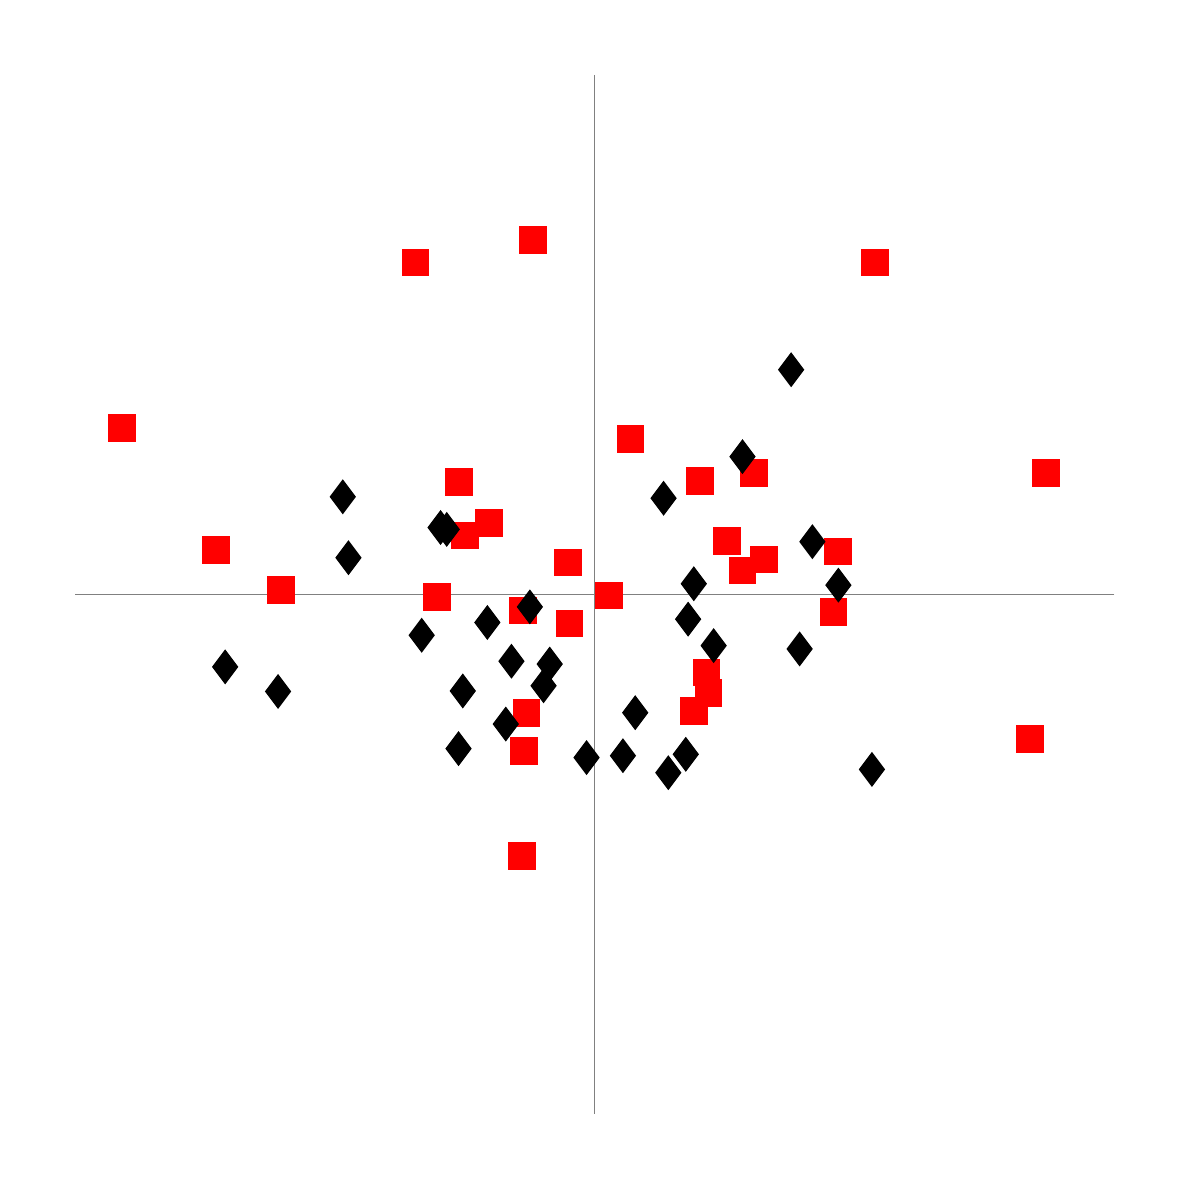
\begin{tikzpicture}[scale=6] \path (-1.2,-1.2) (1.2,1.2);\draw[very thin,color=gray] (0,1.1)--(0,-1.1); \draw[very thin,color=gray] (1.1,0)--(-1.1,0); \path plot[mark=square*,mark options={color=red},mark size=0.8pt] coordinates { (-0.664,0.010) (-0.801,0.094) (0.313,0.051) (-0.144,-0.250) (0.223,0.241) (0.211,-0.246) (-0.333,-0.005) (0.956,0.258) (0.280,0.114) (-0.150,-0.331) (0.515,0.091) (0.030,-0.002) (-0.151,-0.034) (-0.379,0.703) (0.237,-0.165) (-0.224,0.151) (0.338,0.258) (0.594,0.703) (-0.275,0.125) (0.241,-0.208) (0.506,-0.037) (0.921,-0.306) (-0.053,-0.061) (0.359,0.074) (-1.000,0.352) (-0.057,0.068) (-0.153,-0.554) (-0.287,0.239) (0.076,0.330) (-0.130,0.750)};  \path plot[mark=diamond*,mark size=1pt] coordinates { (0.146,0.204) (0.156,-0.377) (-0.670,-0.205) (0.516,0.020) (-0.095,-0.147) (0.461,0.112) (-0.533,0.207) (-0.521,0.078) (0.060,-0.341) (0.434,-0.115) (0.252,-0.108) (-0.108,-0.193) (-0.782,-0.153) (0.086,-0.250) (0.193,-0.338) (-0.137,-0.026) (-0.176,-0.141) (0.210,0.023) (0.416,0.476) (-0.326,0.142) (-0.188,-0.274) (-0.366,-0.086) (-0.227,-0.059) (-0.017,-0.345) (0.587,-0.370) (-0.279,-0.204) (0.198,-0.052) (-0.313,0.138) (0.313,0.292) (-0.288,-0.326)};  \end{tikzpicture} }} & \raisebox{-.5\height}{\resizebox {1.2cm} {1.2cm} { 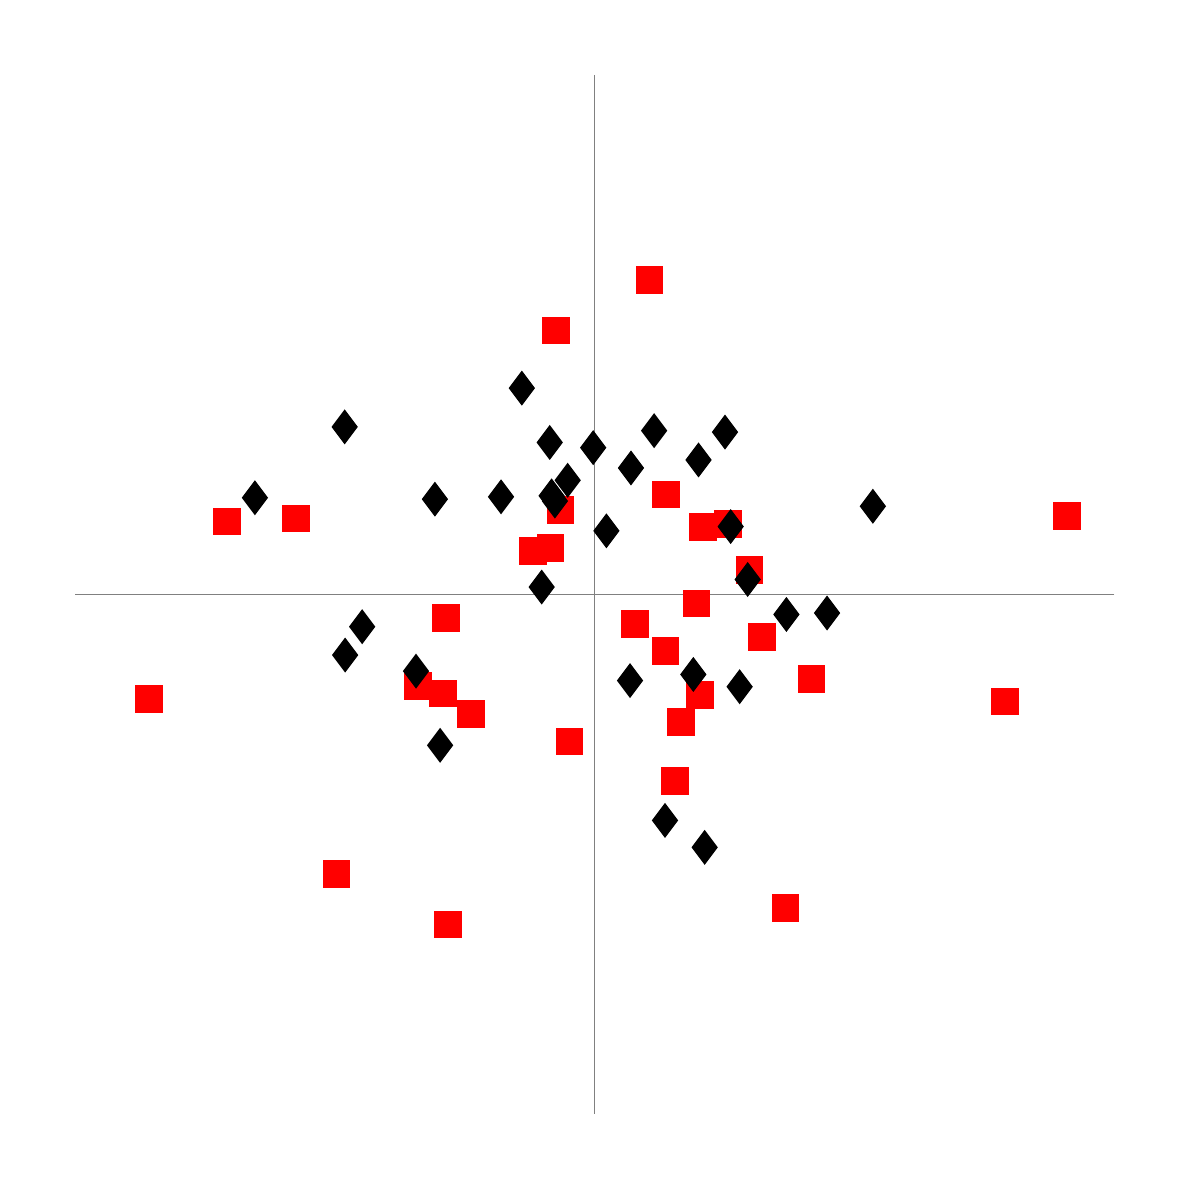
\begin{tikzpicture}[scale=6] \path (-1.2,-1.2) (1.2,1.2);\draw[very thin,color=gray] (0,1.1)--(0,-1.1); \draw[very thin,color=gray] (1.1,0)--(-1.1,0); \path plot[mark=square*,mark options={color=red},mark size=0.8pt] coordinates { (-0.632,0.161) (-0.778,0.155) (0.223,-0.213) (-0.072,0.179) (0.150,-0.120) (0.230,0.143) (-0.315,-0.049) (0.869,-0.226) (0.216,-0.019) (-0.082,0.559) (0.459,-0.179) (0.085,-0.062) (-0.093,0.099) (-0.546,-0.591) (0.328,0.052) (-0.321,-0.209) (0.170,-0.394) (0.404,-0.664) (-0.374,-0.194) (0.282,0.149) (0.354,-0.090) (1.000,0.167) (0.151,0.212) (0.183,-0.269) (-0.943,-0.221) (-0.130,0.092) (0.116,0.666) (-0.262,-0.253) (-0.053,-0.311) (-0.310,-0.698)};  \path plot[mark=diamond*,mark size=1pt] coordinates { (0.075,-0.182) (0.220,0.285) (-0.529,0.355) (0.492,-0.039) (-0.095,0.322) (0.307,-0.195) (-0.528,-0.128) (-0.492,-0.068) (0.077,0.268) (0.406,-0.042) (0.324,0.032) (-0.091,0.209) (-0.719,0.205) (0.126,0.347) (0.276,0.344) (0.025,0.135) (-0.084,0.198) (0.209,-0.169) (0.233,-0.535) (-0.327,-0.319) (-0.057,0.242) (-0.338,0.202) (-0.112,0.016) (-0.003,0.311) (0.589,0.187) (-0.198,0.207) (0.288,0.144) (-0.378,-0.162) (0.149,-0.478) (-0.154,0.437)};  \end{tikzpicture} }} & \raisebox{-.5\height}{\resizebox {1.2cm} {1.2cm} { 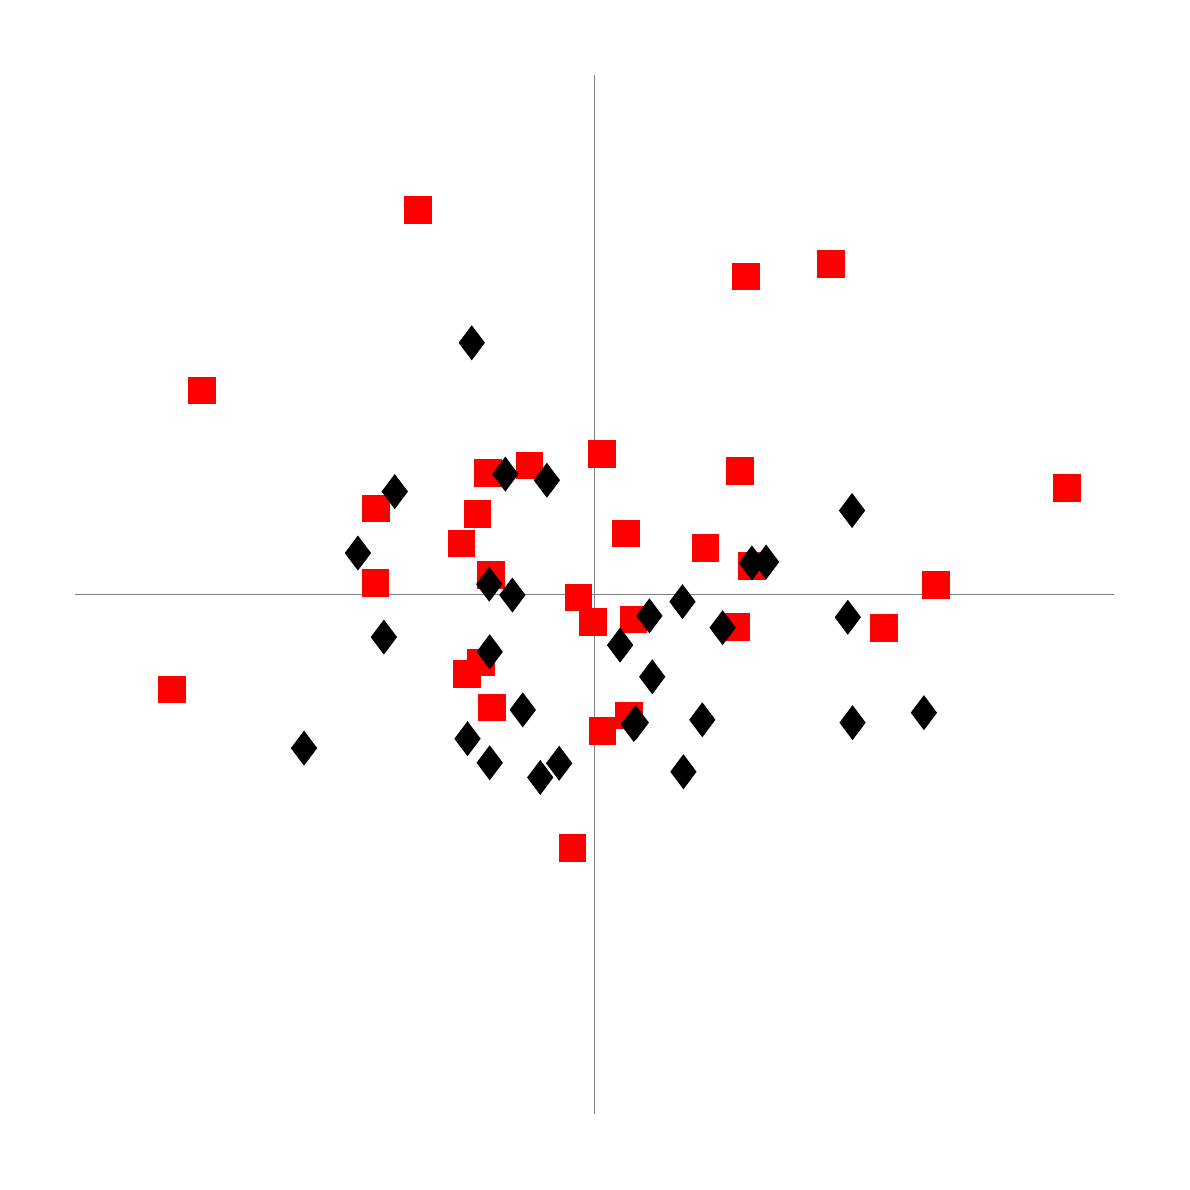
\begin{tikzpicture}[scale=6] \path (-1.2,-1.2) (1.2,1.2);\draw[very thin,color=gray] (0,1.1)--(0,-1.1); \draw[very thin,color=gray] (1.1,0)--(-1.1,0); \path plot[mark=square*,mark options={color=red},mark size=0.8pt] coordinates { (0.613,-0.071) (0.723,0.021) (-0.219,0.042) (0.073,-0.256) (-0.138,0.273) (-0.217,-0.239) (0.300,-0.069) (-0.831,0.432) (-0.248,0.171) (0.017,-0.289) (-0.462,0.182) (-0.034,-0.006) (0.082,-0.053) (0.501,0.700) (-0.241,-0.144) (0.235,0.098) (-0.226,0.258) (-0.374,0.814) (0.333,0.060) (-0.270,-0.168) (-0.464,0.025) (-0.895,-0.201) (-0.004,-0.058) (-0.282,0.108) (1.000,0.225) (0.066,0.129) (-0.047,-0.537) (0.308,0.262) (0.015,0.298) (0.321,0.673)};  \path plot[mark=diamond*,mark size=1pt] coordinates { (-0.101,0.242) (-0.222,-0.356) (0.546,-0.271) (-0.501,0.088) (0.054,-0.107) (-0.423,0.218) (0.545,0.178) (0.536,-0.048) (-0.115,-0.387) (-0.446,-0.090) (-0.222,-0.121) (0.087,-0.271) (0.697,-0.250) (-0.152,-0.244) (-0.269,-0.305) (0.116,-0.045) (0.122,-0.174) (-0.174,-0.001) (-0.260,0.533) (0.333,0.067) (0.083,-0.275) (0.271,-0.070) (0.186,-0.015) (-0.075,-0.357) (-0.615,-0.325) (0.228,-0.265) (-0.223,0.022) (0.363,0.069) (-0.189,0.255) (0.188,-0.375)};  \end{tikzpicture} }} & \raisebox{-.5\height}{\resizebox {1.2cm} {1.2cm} { 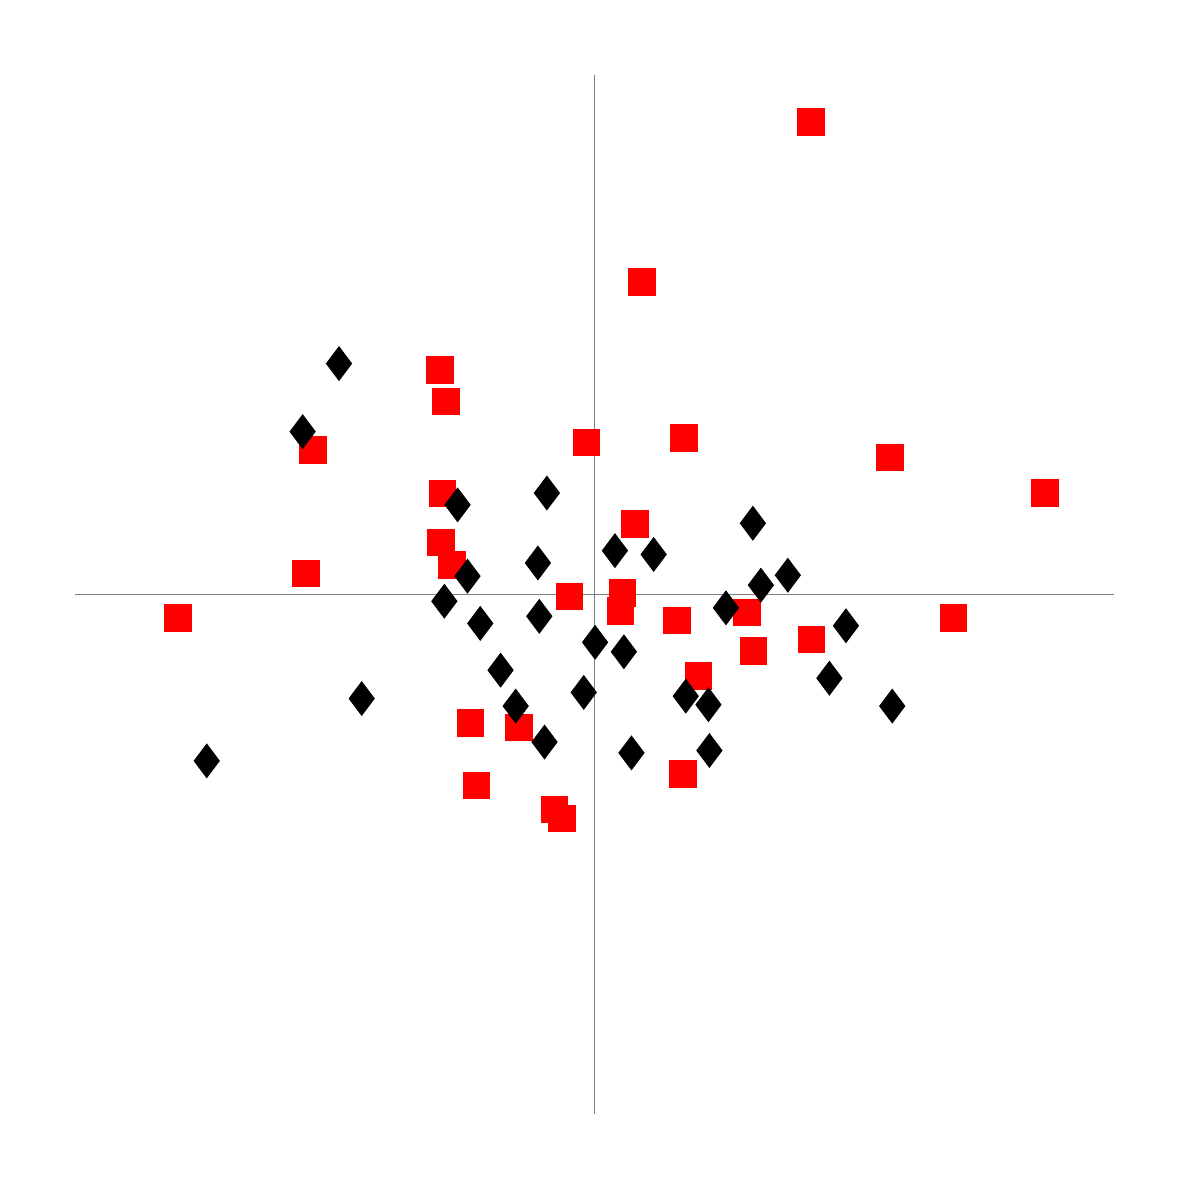
\begin{tikzpicture}[scale=6] \path (-1.2,-1.2) (1.2,1.2);\draw[very thin,color=gray] (0,1.1)--(0,-1.1); \draw[very thin,color=gray] (1.1,0)--(-1.1,0); \path plot[mark=square*,mark options={color=red},mark size=0.8pt] coordinates { (0.760,-0.049) (0.625,0.290) (-0.263,-0.272) (0.187,-0.380) (-0.314,0.409) (-0.069,-0.474) (0.459,-0.095) (-0.596,0.306) (-0.322,0.214) (0.055,-0.035) (-0.302,0.062) (-0.053,-0.004) (0.322,-0.038) (0.458,1.000) (-0.085,-0.455) (0.086,0.150) (-0.325,0.110) (-0.327,0.476) (0.336,-0.119) (-0.160,-0.281) (-0.611,0.045) (-0.882,-0.050) (0.174,-0.055) (-0.250,-0.404) (0.954,0.215) (0.059,0.003) (0.220,-0.172) (0.189,0.332) (-0.017,0.322) (0.101,0.662)};  \path plot[mark=diamond*,mark size=1pt] coordinates { (-0.101,0.215) (-0.167,-0.236) (0.630,-0.236) (-0.618,0.345) (-0.120,0.067) (-0.318,-0.014) (0.409,0.041) (0.497,-0.177) (-0.106,-0.312) (-0.269,0.039) (-0.199,-0.160) (0.078,-0.335) (0.532,-0.066) (-0.242,-0.061) (-0.493,-0.220) (0.125,0.085) (0.001,-0.101) (-0.117,-0.046) (-0.541,0.489) (0.352,0.020) (0.062,-0.121) (0.335,0.151) (0.278,-0.028) (-0.023,-0.207) (-0.821,-0.352) (0.243,-0.330) (0.043,0.093) (0.241,-0.233) (-0.290,0.190) (0.193,-0.215)};  \end{tikzpicture} }} & \raisebox{-.5\height}{\resizebox {1.2cm} {1.2cm} { 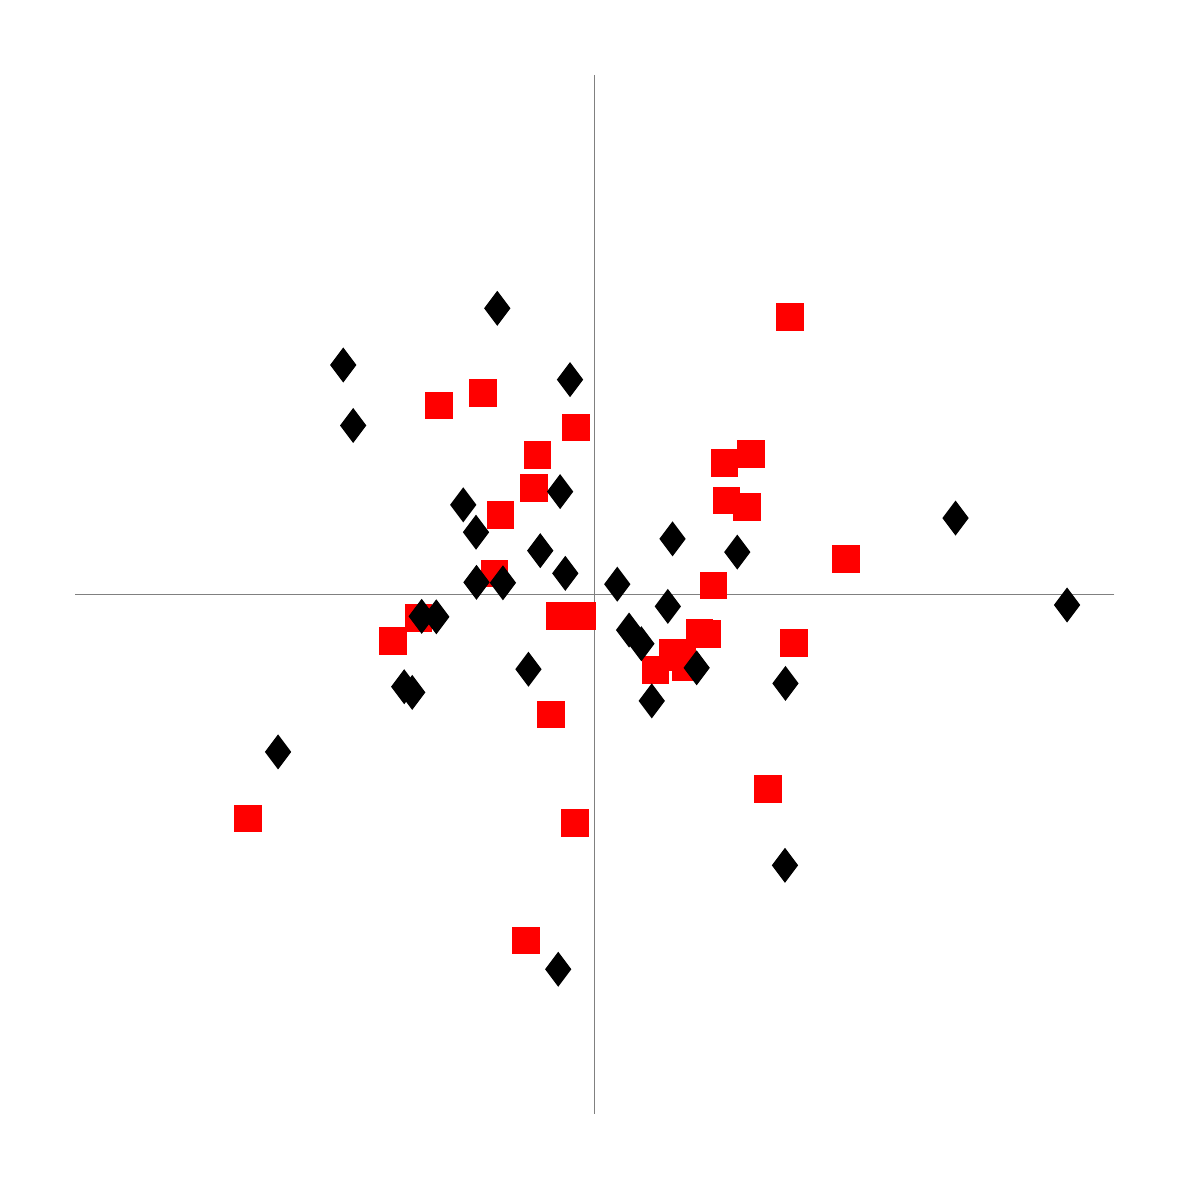
\begin{tikzpicture}[scale=6] \path (-1.2,-1.2) (1.2,1.2);\draw[very thin,color=gray] (0,1.1)--(0,-1.1); \draw[very thin,color=gray] (1.1,0)--(-1.1,0); \path plot[mark=square*,mark options={color=red},mark size=0.8pt] coordinates { (0.239,-0.084) (-0.329,0.400) (-0.040,0.354) (0.252,0.019) (0.166,-0.123) (0.322,0.185) (0.422,-0.103) (0.186,-0.133) (0.275,0.279) (0.367,-0.412) (-0.236,0.427) (-0.042,-0.484) (0.129,-0.160) (-0.145,-0.732) (0.279,0.199) (-0.128,0.225) (-0.199,0.168) (-0.121,0.295) (-0.427,-0.098) (-0.092,-0.254) (0.194,-0.154) (0.414,0.588) (0.532,0.075) (0.331,0.297) (-0.026,-0.045) (-0.212,0.045) (-0.373,-0.050) (-0.734,-0.474) (-0.073,-0.045) (0.222,-0.081)};  \path plot[mark=diamond*,mark size=1pt] coordinates { (-0.511,0.358) (0.764,0.162) (0.216,-0.155) (0.403,-0.573) (0.121,-0.225) (-0.250,0.026) (-0.335,-0.047) (1.000,-0.022) (-0.278,0.190) (0.155,-0.025) (0.048,0.022) (-0.052,0.455) (-0.073,0.218) (-0.403,-0.195) (0.099,-0.104) (0.302,0.090) (-0.386,-0.207) (-0.194,0.025) (-0.062,0.045) (-0.366,-0.046) (-0.251,0.132) (-0.670,-0.333) (-0.140,-0.158) (-0.532,0.486) (-0.206,0.606) (-0.077,-0.793) (0.073,-0.075) (0.404,-0.188) (0.165,0.118) (-0.115,0.093)};  \end{tikzpicture} }} & \raisebox{-.5\height}{\resizebox {1.2cm} {1.2cm} { 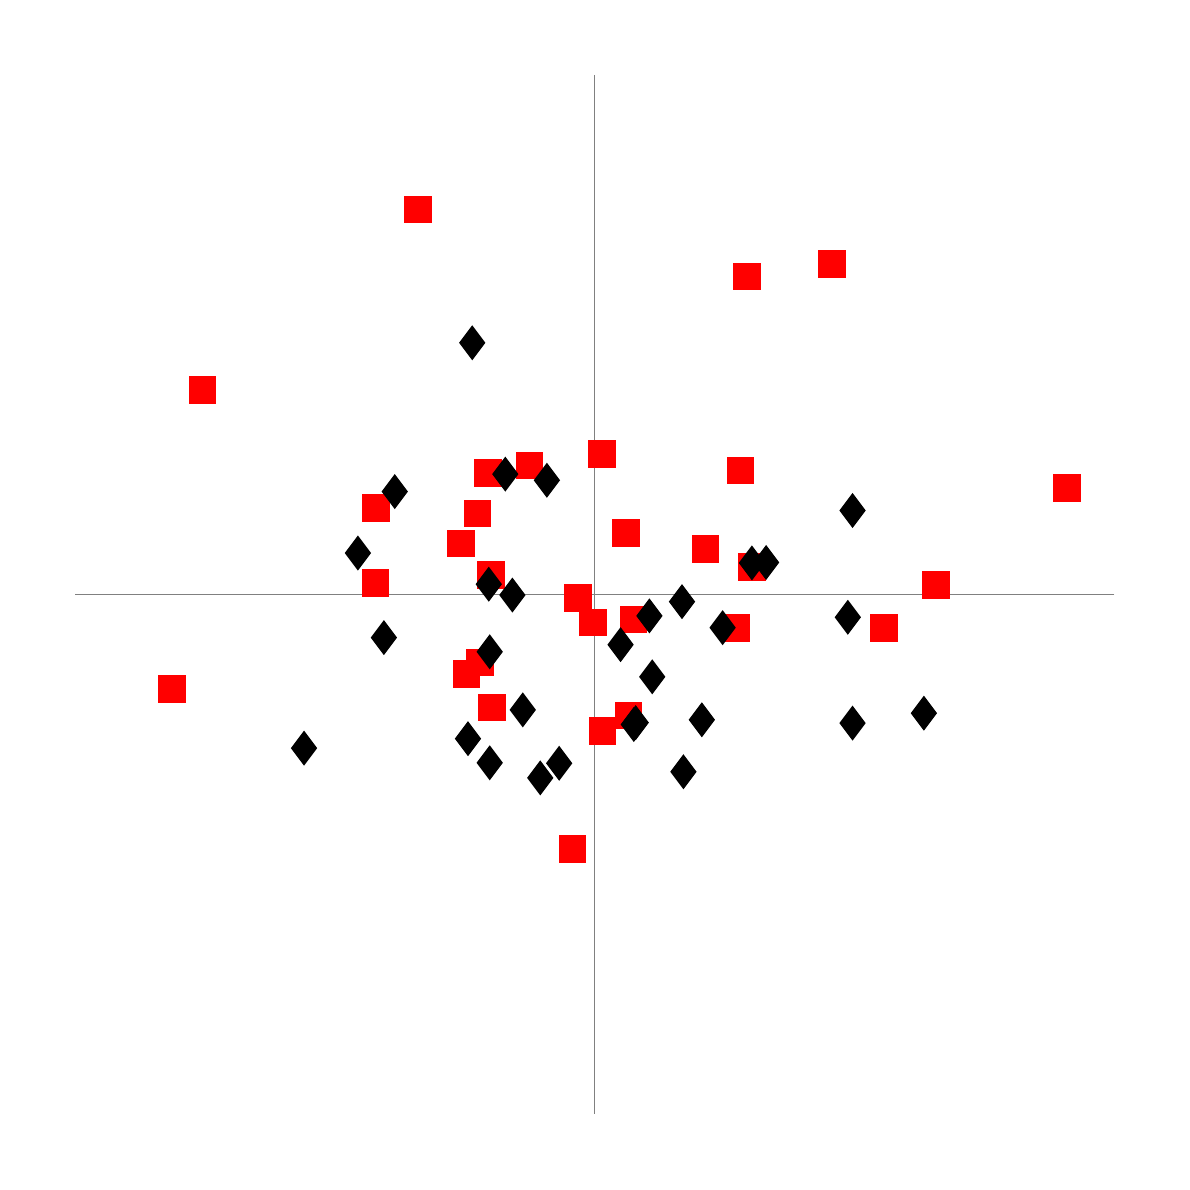
\begin{tikzpicture}[scale=6] \path (-1.2,-1.2) (1.2,1.2);\draw[very thin,color=gray] (0,1.1)--(0,-1.1); \draw[very thin,color=gray] (1.1,0)--(-1.1,0); \path plot[mark=square*,mark options={color=red},mark size=0.8pt] coordinates { (0.613,-0.071) (0.723,0.021) (-0.219,0.042) (0.072,-0.256) (-0.138,0.273) (-0.217,-0.239) (0.300,-0.070) (-0.830,0.433) (-0.248,0.172) (0.017,-0.289) (-0.462,0.183) (-0.035,-0.007) (0.082,-0.053) (0.502,0.700) (-0.242,-0.144) (0.235,0.097) (-0.226,0.258) (-0.374,0.815) (0.333,0.059) (-0.271,-0.168) (-0.464,0.025) (-0.895,-0.200) (-0.004,-0.059) (-0.283,0.108) (1.000,0.225) (0.066,0.130) (-0.047,-0.538) (0.309,0.263) (0.015,0.298) (0.322,0.673)};  \path plot[mark=diamond*,mark size=1pt] coordinates { (-0.101,0.242) (-0.222,-0.356) (0.546,-0.272) (-0.501,0.088) (0.055,-0.106) (-0.423,0.218) (0.546,0.178) (0.536,-0.048) (-0.115,-0.388) (-0.446,-0.091) (-0.222,-0.121) (0.087,-0.271) (0.697,-0.251) (-0.152,-0.244) (-0.268,-0.305) (0.116,-0.045) (0.122,-0.174) (-0.174,-0.001) (-0.259,0.533) (0.333,0.067) (0.083,-0.275) (0.271,-0.070) (0.185,-0.015) (-0.075,-0.357) (-0.615,-0.325) (0.227,-0.265) (-0.224,0.022) (0.363,0.068) (-0.189,0.255) (0.188,-0.375)};  \end{tikzpicture} }} & \raisebox{-.5\height}{\resizebox {1.2cm} {1.2cm} { 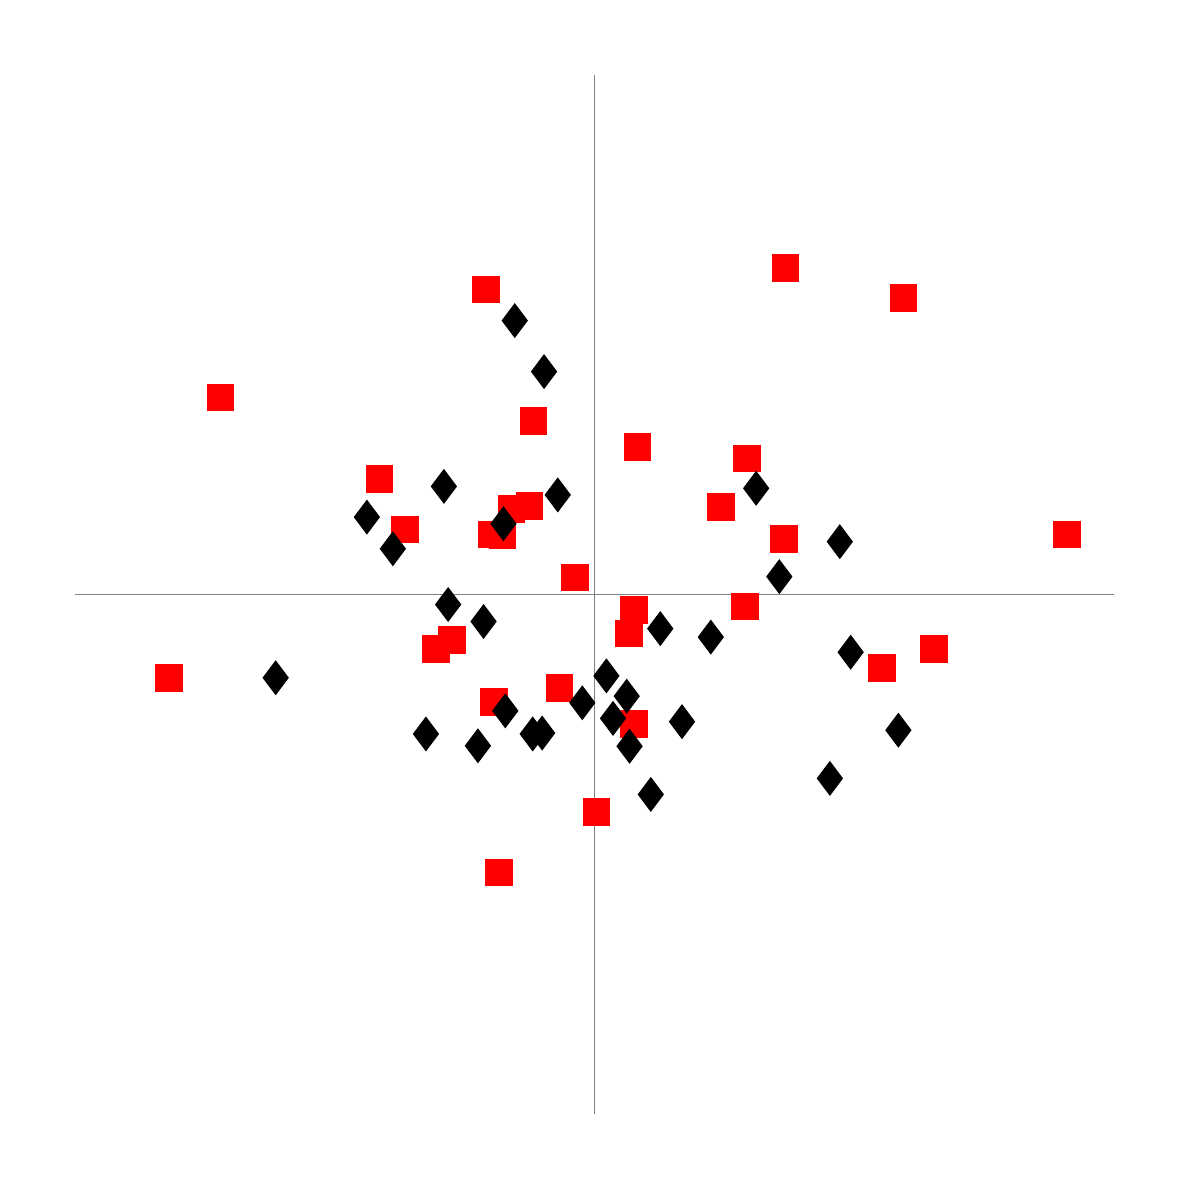
\begin{tikzpicture}[scale=6] \path (-1.2,-1.2) (1.2,1.2);\draw[very thin,color=gray] (0,1.1)--(0,-1.1); \draw[very thin,color=gray] (1.1,0)--(-1.1,0); \path plot[mark=square*,mark options={color=red},mark size=0.8pt] coordinates { (0.609,-0.155) (0.718,-0.115) (-0.195,0.125) (0.083,-0.274) (-0.138,0.188) (-0.213,-0.228) (0.319,-0.025) (-0.792,0.417) (-0.217,0.127) (0.004,-0.460) (-0.455,0.245) (-0.041,0.036) (0.073,-0.082) (0.654,0.628) (-0.302,-0.096) (0.267,0.185) (-0.129,0.368) (-0.230,0.646) (0.401,0.117) (-0.336,-0.115) (-0.402,0.138) (-0.901,-0.176) (-0.074,-0.198) (-0.176,0.181) (1.000,0.127) (0.083,-0.032) (-0.203,-0.588) (0.322,0.288) (0.091,0.313) (0.404,0.691)};  \path plot[mark=diamond*,mark size=1pt] coordinates { (-0.078,0.211) (-0.247,-0.320) (0.498,-0.389) (-0.482,0.164) (0.039,-0.262) (-0.319,0.229) (0.519,0.112) (0.542,-0.122) (-0.131,-0.295) (-0.427,0.097) (-0.310,-0.021) (0.074,-0.321) (0.643,-0.287) (-0.189,-0.246) (-0.357,-0.295) (0.025,-0.172) (0.068,-0.215) (-0.193,0.150) (-0.169,0.580) (0.342,0.225) (-0.026,-0.229) (0.246,-0.090) (0.139,-0.072) (-0.111,-0.293) (-0.675,-0.176) (0.185,-0.269) (-0.235,-0.057) (0.391,0.038) (-0.107,0.472) (0.119,-0.423)};  \end{tikzpicture} }}\\
\midrule
\multirow{4}{*}{II}
 & $\#$PCs & 13 & 15 & 13 & 1 & 28 & 14 & 21\\
 & MNV & \uuline{4e-05} & \uuline{<1e-08} & \uuline{0.002} & * & 0.089 & \uuline{0.003} & \uuline{2e-07}\\
 & $t$-test & \uline{0.042} & \uuline{<1e-08} & 0.108 & \uuline{<1e-08} & \uline{0.017} & 0.109 & 0.390\\
 & PCS & \raisebox{-.5\height}{\resizebox {1.2cm} {1.2cm} { 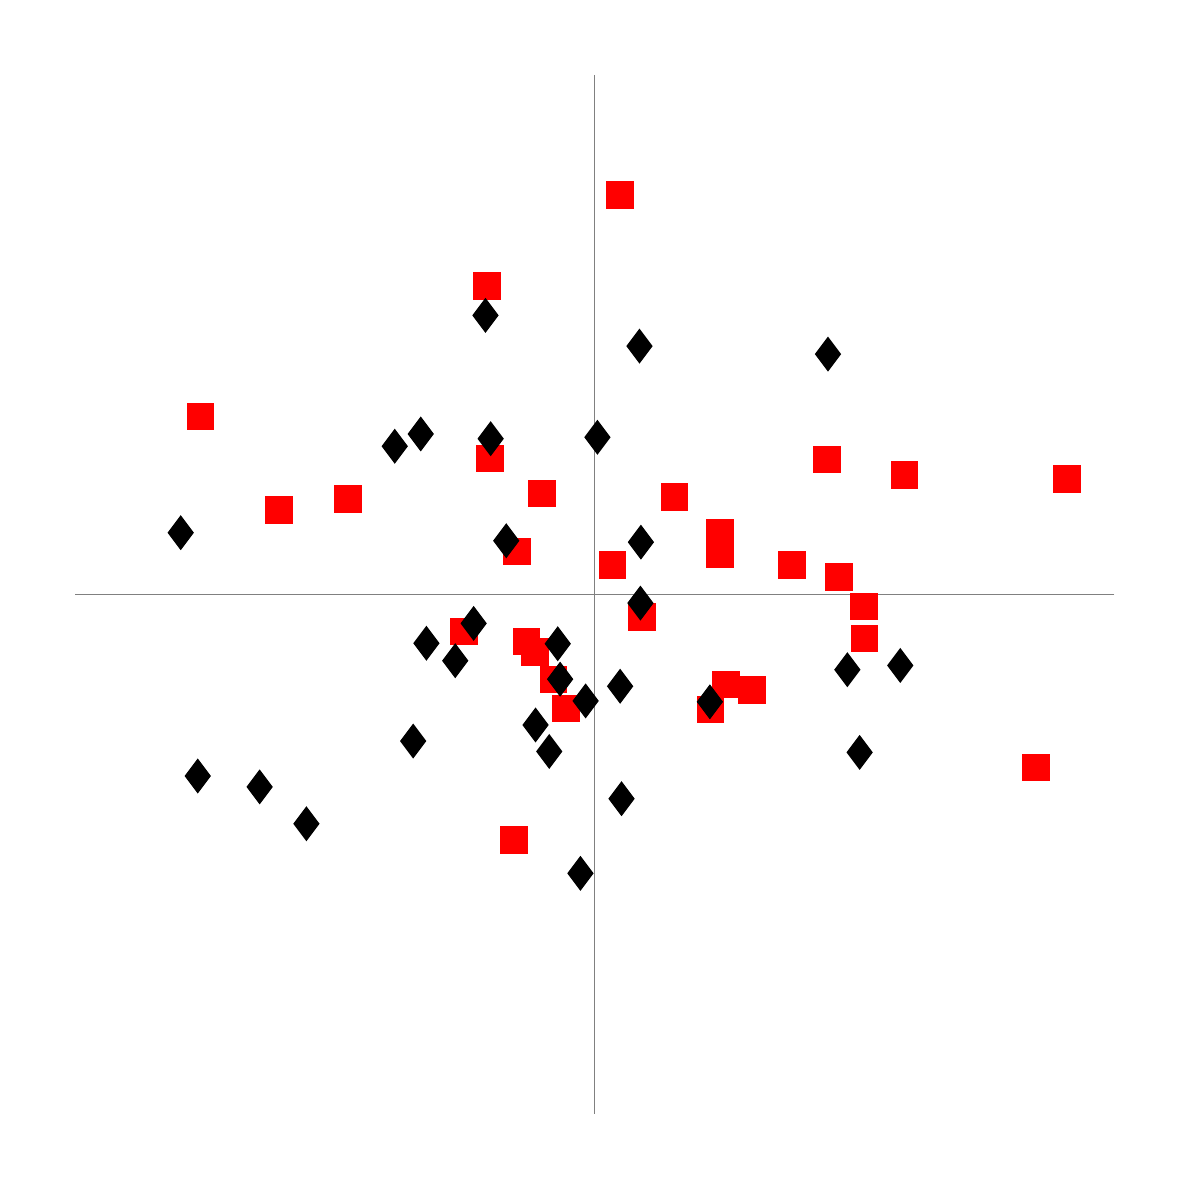
\begin{tikzpicture}[scale=6] \path (-1.2,-1.2) (1.2,1.2);\draw[very thin,color=gray] (0,1.1)--(0,-1.1); \draw[very thin,color=gray] (1.1,0)--(-1.1,0); \path plot[mark=square*,mark options={color=red},mark size=0.8pt] coordinates { (-0.522,0.202) (-0.668,0.179) (0.418,0.063) (-0.061,-0.241) (0.266,0.131) (0.333,-0.202) (-0.276,-0.078) (1.000,0.245) (0.265,0.086) (-0.126,-0.121) (0.570,-0.025) (0.100,-0.048) (-0.144,-0.099) (-0.228,0.653) (0.245,-0.243) (-0.164,0.091) (0.492,0.286) (0.656,0.253) (-0.112,0.214) (0.278,-0.190) (0.571,-0.093) (0.935,-0.366) (-0.087,-0.180) (0.517,0.037) (-0.834,0.377) (0.038,0.063) (-0.171,-0.519) (-0.222,0.288) (0.169,0.207) (0.054,0.846)};  \path plot[mark=diamond*,mark size=1pt] coordinates { (0.098,0.111) (-0.030,-0.590) (0.006,0.333) (0.494,0.509) (-0.423,0.314) (-0.610,-0.485) (-0.187,0.114) (-0.840,-0.384) (-0.019,-0.225) (-0.125,-0.276) (-0.231,0.591) (-0.876,0.131) (-0.256,-0.061) (-0.384,-0.310) (0.647,-0.150) (-0.220,0.330) (-0.356,-0.103) (0.244,-0.227) (-0.073,-0.179) (-0.709,-0.407) (0.097,-0.018) (-0.096,-0.332) (-0.368,0.340) (0.561,-0.334) (-0.295,-0.140) (0.057,-0.432) (-0.078,-0.104) (0.054,-0.194) (0.535,-0.159) (0.095,0.526)};  \end{tikzpicture} }} & \raisebox{-.5\height}{\resizebox {1.2cm} {1.2cm} { 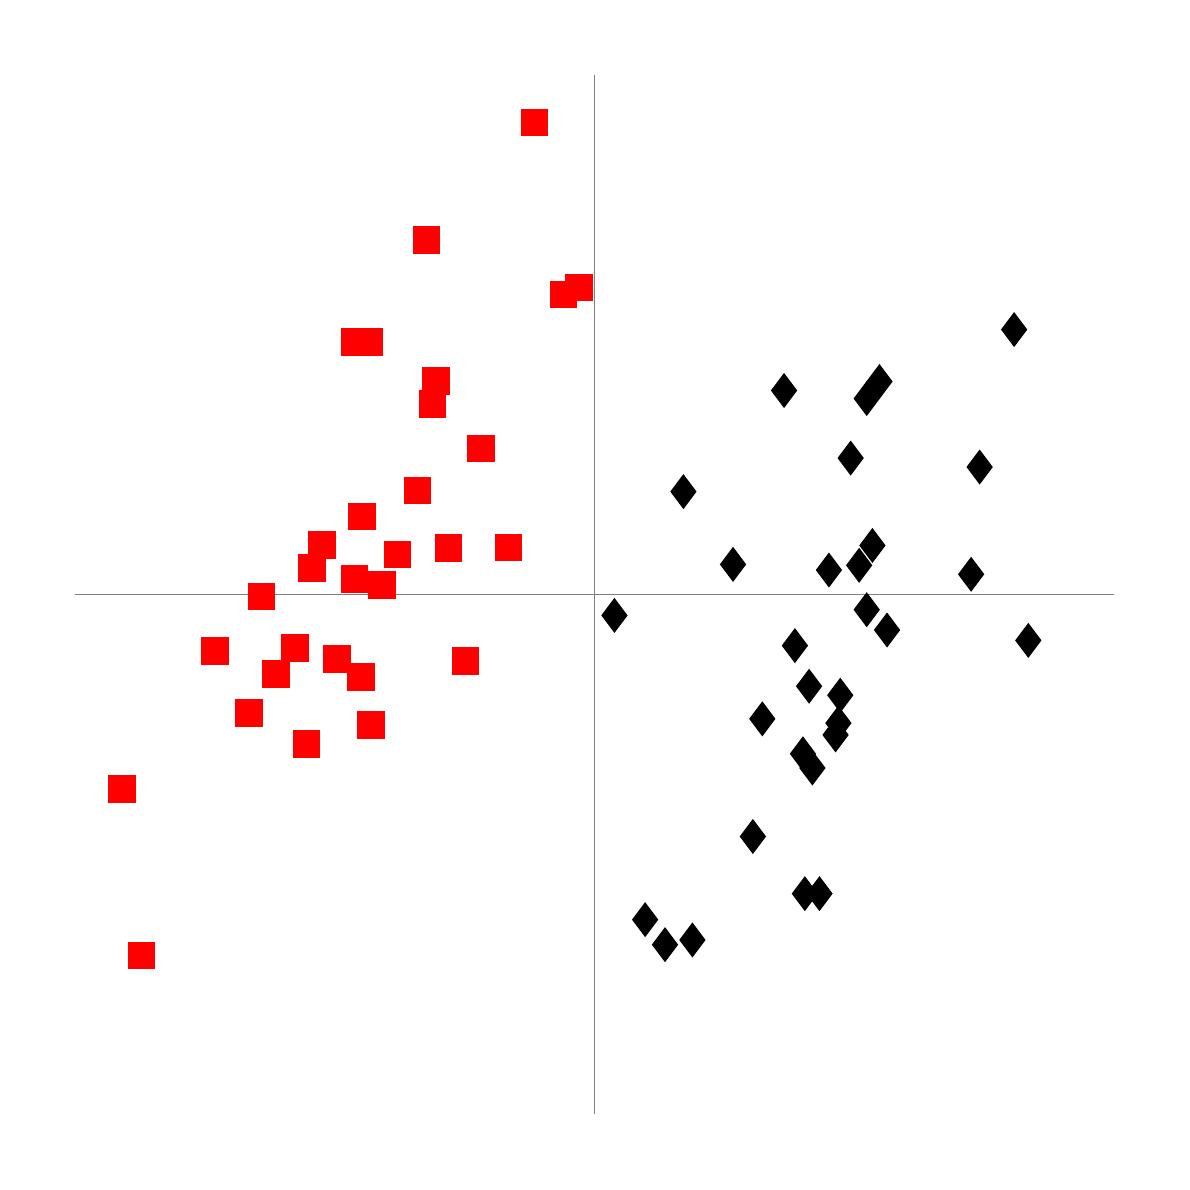
\begin{tikzpicture}[scale=6] \path (-1.2,-1.2) (1.2,1.2);\draw[very thin,color=gray] (0,1.1)--(0,-1.1); \draw[very thin,color=gray] (1.1,0)--(-1.1,0); \path plot[mark=square*,mark options={color=red},mark size=0.8pt] coordinates { (-0.066,0.635) (-0.033,0.650) (-0.634,-0.113) (-0.417,0.085) (-0.598,0.057) (-0.473,-0.276) (-0.241,0.309) (-1.000,-0.412) (-0.577,0.105) (-0.182,0.100) (-0.732,-0.251) (-0.508,0.033) (-0.375,0.220) (-0.356,0.750) (-0.545,-0.137) (-0.336,0.452) (-0.705,-0.004) (-0.804,-0.119) (-0.343,0.404) (-0.494,-0.174) (-0.610,-0.316) (-0.959,-0.764) (-0.450,0.020) (-0.675,-0.168) (-0.127,0.999) (-0.309,0.098) (-0.273,-0.141) (-0.478,0.535) (-0.493,0.165) (-0.507,0.534)};  \path plot[mark=diamond*,mark size=1pt] coordinates { (0.424,-0.108) (0.476,-0.633) (0.293,0.064) (0.042,-0.044) (0.603,0.451) (0.918,-0.097) (0.560,0.062) (0.815,0.270) (0.510,-0.297) (0.516,-0.272) (0.576,0.415) (0.888,0.561) (0.496,0.052) (0.619,-0.075) (0.149,-0.741) (0.542,0.289) (0.588,0.104) (0.445,-0.633) (0.520,-0.213) (0.797,0.043) (0.355,-0.263) (0.441,-0.337) (0.401,0.432) (0.207,-0.731) (0.576,-0.032) (0.335,-0.512) (0.454,-0.194) (0.461,-0.367) (0.107,-0.688) (0.188,0.218)};  \end{tikzpicture} }} & \raisebox{-.5\height}{\resizebox {1.2cm} {1.2cm} { 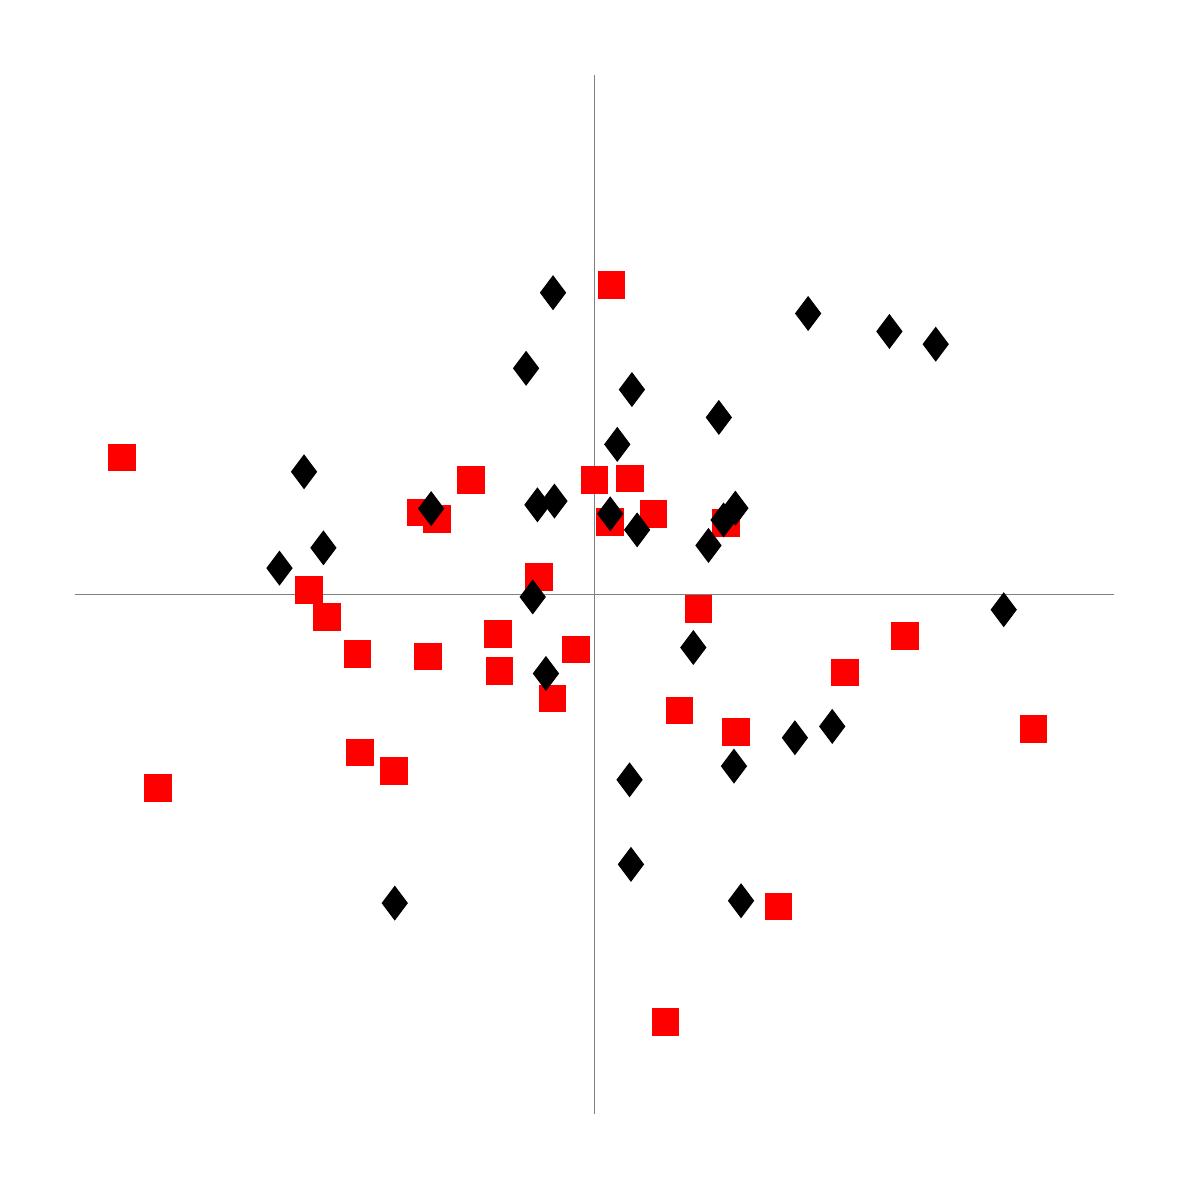
\begin{tikzpicture}[scale=6] \path (-1.2,-1.2) (1.2,1.2);\draw[very thin,color=gray] (0,1.1)--(0,-1.1); \draw[very thin,color=gray] (1.1,0)--(-1.1,0); \path plot[mark=square*,mark options={color=red},mark size=0.8pt] coordinates { (0.530,-0.165) (0.657,-0.087) (-0.352,-0.131) (-0.000,0.243) (-0.201,-0.162) (-0.368,0.174) (0.278,0.152) (-0.924,-0.409) (-0.204,-0.083) (0.033,0.154) (-0.567,-0.047) (-0.118,0.037) (0.125,0.171) (0.389,-0.660) (-0.261,0.242) (0.220,-0.031) (-0.424,-0.374) (-0.496,-0.334) (0.180,-0.245) (-0.334,0.160) (-0.605,0.010) (-1.000,0.290) (0.075,0.246) (-0.502,-0.126) (0.929,-0.285) (-0.039,-0.116) (0.036,0.655) (0.300,-0.291) (-0.089,-0.220) (0.150,-0.905)};  \path plot[mark=diamond*,mark size=1pt] coordinates { (-0.103,-0.167) (-0.088,0.639) (0.074,-0.392) (-0.423,-0.653) (0.503,-0.279) (0.452,0.595) (0.209,-0.112) (0.722,0.530) (-0.085,0.198) (0.048,0.318) (0.310,-0.648) (0.866,-0.032) (0.241,0.104) (0.263,0.375) (-0.667,0.056) (0.295,-0.363) (0.273,0.158) (-0.346,0.182) (0.033,0.171) (0.624,0.557) (-0.131,-0.005) (0.079,0.434) (0.424,-0.303) (-0.615,0.260) (0.298,0.183) (-0.145,0.479) (0.090,0.137) (-0.121,0.190) (-0.574,0.099) (0.077,-0.571)};  \end{tikzpicture} }} & \raisebox{-.5\height}{\resizebox {1.2cm} {1.2cm} { 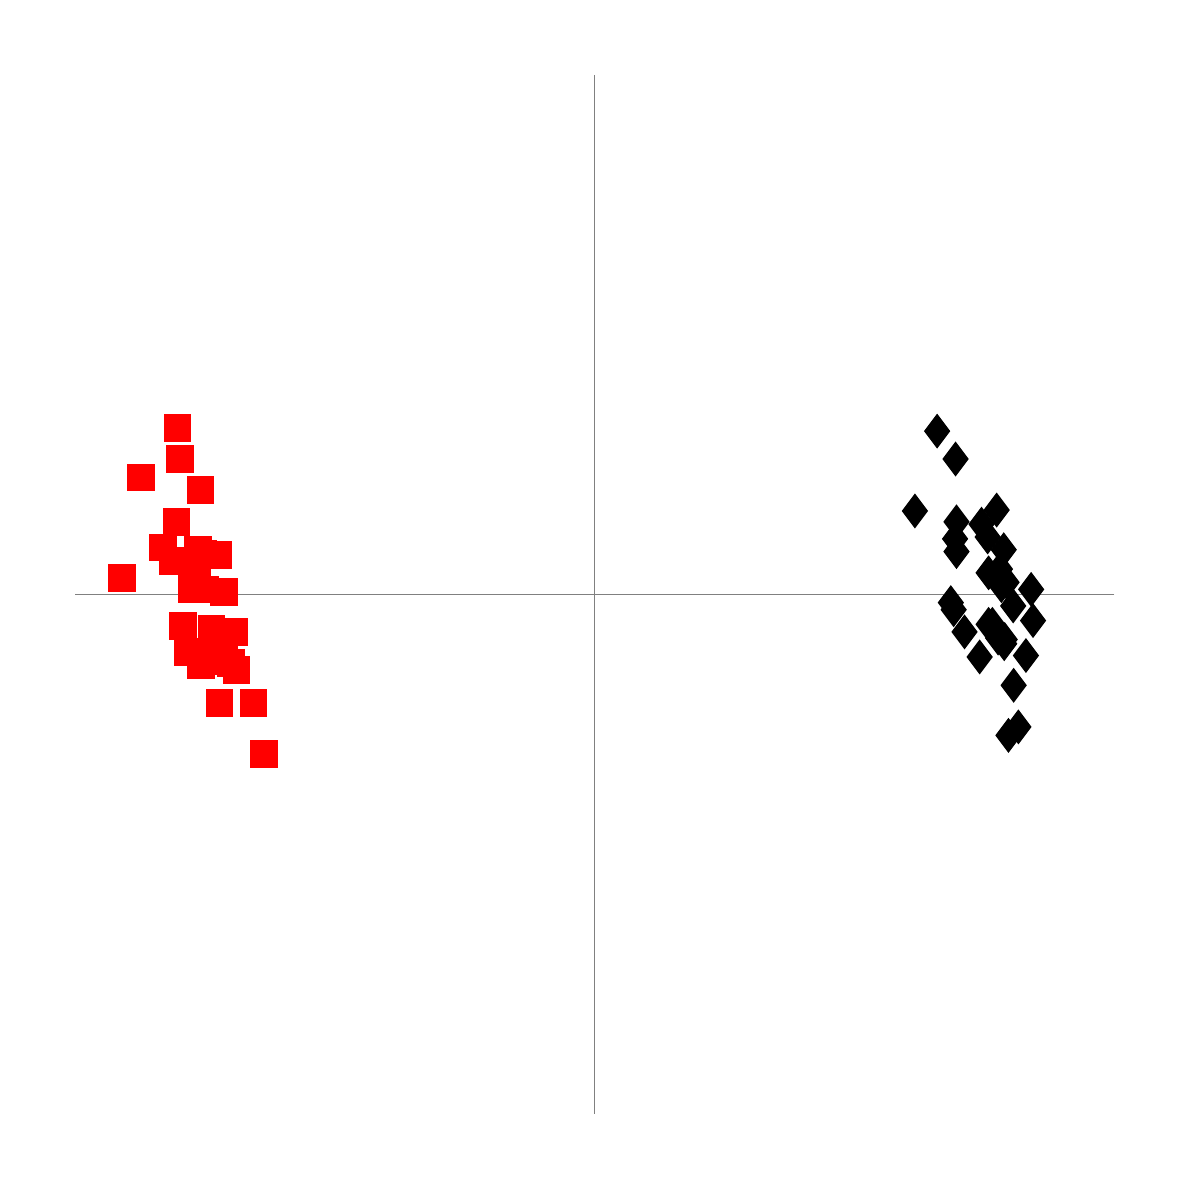
\begin{tikzpicture}[scale=6] \path (-1.2,-1.2) (1.2,1.2);\draw[very thin,color=gray] (0,1.1)--(0,-1.1); \draw[very thin,color=gray] (1.1,0)--(-1.1,0); \path plot[mark=square*,mark options={color=red},mark size=0.8pt] coordinates { (-0.877,0.287) (-0.960,0.248) (-0.815,-0.141) (-0.824,0.011) (-0.763,-0.079) (-0.784,-0.112) (-0.885,0.154) (-0.722,-0.229) (-0.861,-0.121) (-0.850,0.063) (-0.791,-0.134) (-0.871,-0.066) (-0.914,0.100) (-0.834,0.222) (-0.811,-0.073) (-0.841,0.039) (-0.833,-0.150) (-0.769,-0.145) (-0.893,0.071) (-0.809,-0.102) (-0.794,-0.230) (-0.700,-0.337) (-0.796,0.084) (-0.758,-0.160) (-0.883,0.353) (-0.853,0.012) (-1.000,0.035) (-0.839,0.094) (-0.784,0.005) (-0.828,0.086)};  \path plot[mark=diamond*,mark size=1pt] coordinates { (0.783,-0.079) (0.815,-0.132) (0.858,0.054) (0.913,-0.129) (0.851,0.179) (0.832,0.122) (0.861,0.019) (0.764,0.287) (0.928,-0.055) (0.924,0.011) (0.766,0.154) (0.725,0.346) (0.754,-0.017) (0.766,0.091) (0.887,-0.192) (0.866,0.095) (0.763,0.118) (0.867,-0.104) (0.842,-0.063) (0.678,0.177) (0.868,-0.095) (0.760,-0.032) (0.819,0.149) (0.876,-0.298) (0.834,0.046) (0.854,-0.092) (0.872,0.026) (0.834,-0.063) (0.897,-0.280) (0.886,-0.024)};  \end{tikzpicture} }} & \raisebox{-.5\height}{\resizebox {1.2cm} {1.2cm} { 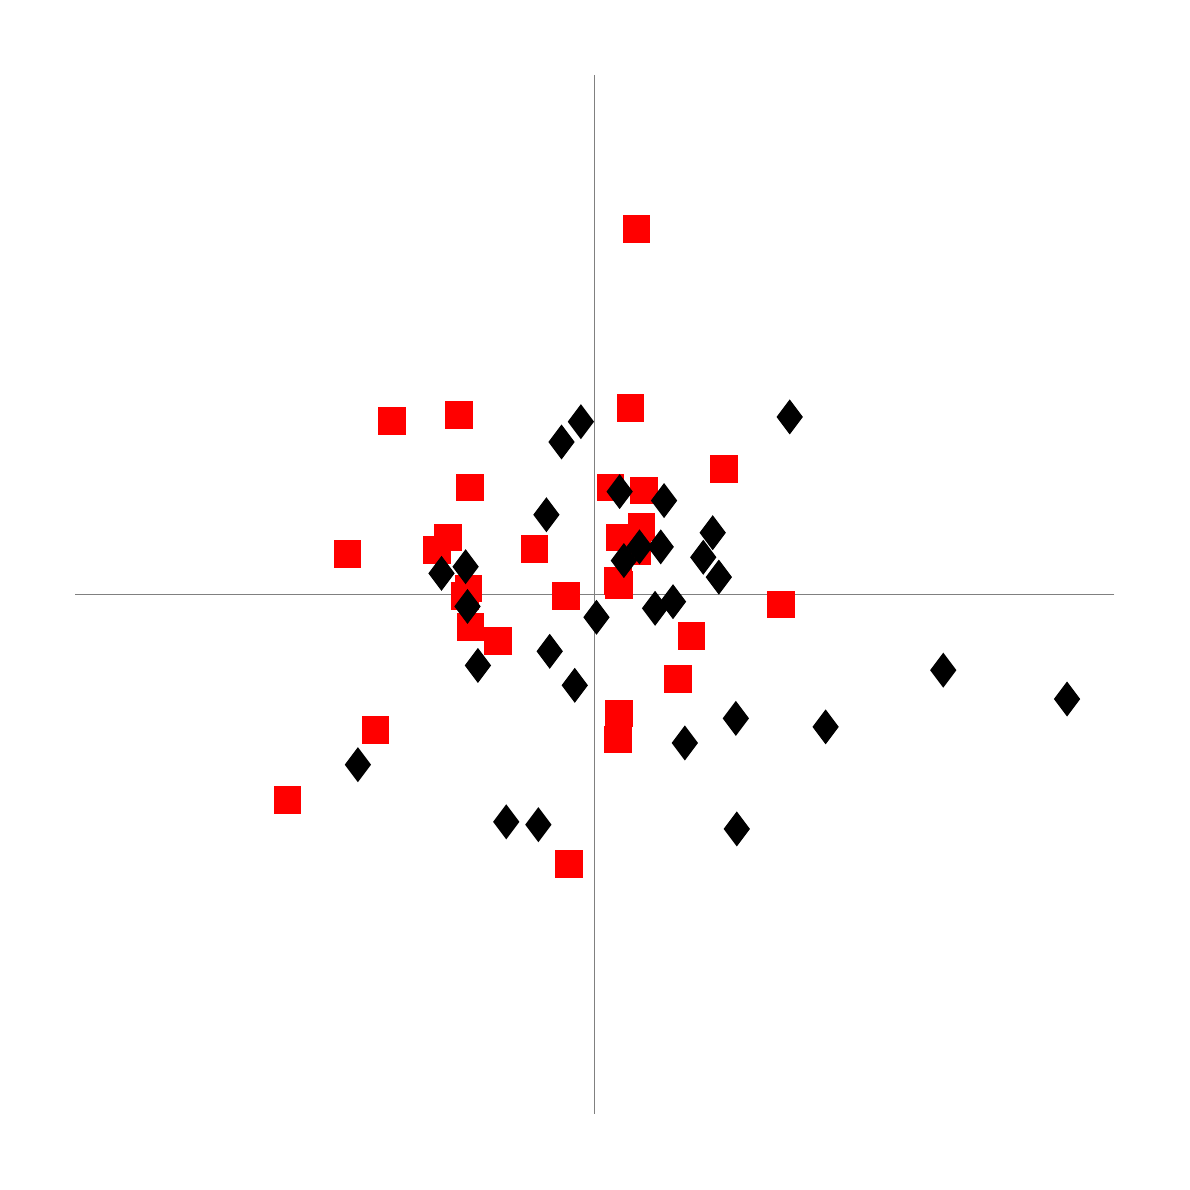
\begin{tikzpicture}[scale=6] \path (-1.2,-1.2) (1.2,1.2);\draw[very thin,color=gray] (0,1.1)--(0,-1.1); \draw[very thin,color=gray] (1.1,0)--(-1.1,0); \path plot[mark=square*,mark options={color=red},mark size=0.8pt] coordinates { (0.177,-0.178) (-0.523,0.086) (-0.287,0.380) (0.090,0.092) (0.054,0.121) (0.099,0.143) (0.205,-0.088) (0.049,0.029) (0.034,0.227) (0.395,-0.021) (-0.429,0.368) (0.050,-0.307) (-0.060,-0.003) (-0.054,-0.570) (0.076,0.395) (-0.333,0.095) (-0.274,-0.003) (-0.311,0.121) (-0.464,-0.286) (-0.127,0.097) (0.052,0.021) (0.089,0.774) (0.274,0.266) (0.104,0.220) (-0.204,-0.098) (-0.267,0.013) (-0.264,0.227) (-0.650,-0.435) (-0.263,-0.069) (0.051,-0.252)};  \path plot[mark=diamond*,mark size=1pt] coordinates { (-0.269,-0.025) (0.413,0.376) (0.489,-0.280) (-0.119,-0.487) (0.299,-0.262) (1.000,-0.221) (0.004,-0.048) (-0.273,0.059) (0.147,0.199) (0.140,0.101) (-0.501,-0.360) (-0.095,-0.120) (0.095,0.101) (0.263,0.037) (0.738,-0.160) (-0.247,-0.150) (0.230,0.079) (-0.029,0.366) (0.191,-0.314) (-0.324,0.045) (-0.042,-0.192) (0.128,-0.029) (0.301,-0.496) (-0.070,0.323) (0.250,0.131) (0.062,0.072) (-0.102,0.169) (0.053,0.218) (0.166,-0.015) (-0.187,-0.481)};  \end{tikzpicture} }} & \raisebox{-.5\height}{\resizebox {1.2cm} {1.2cm} { 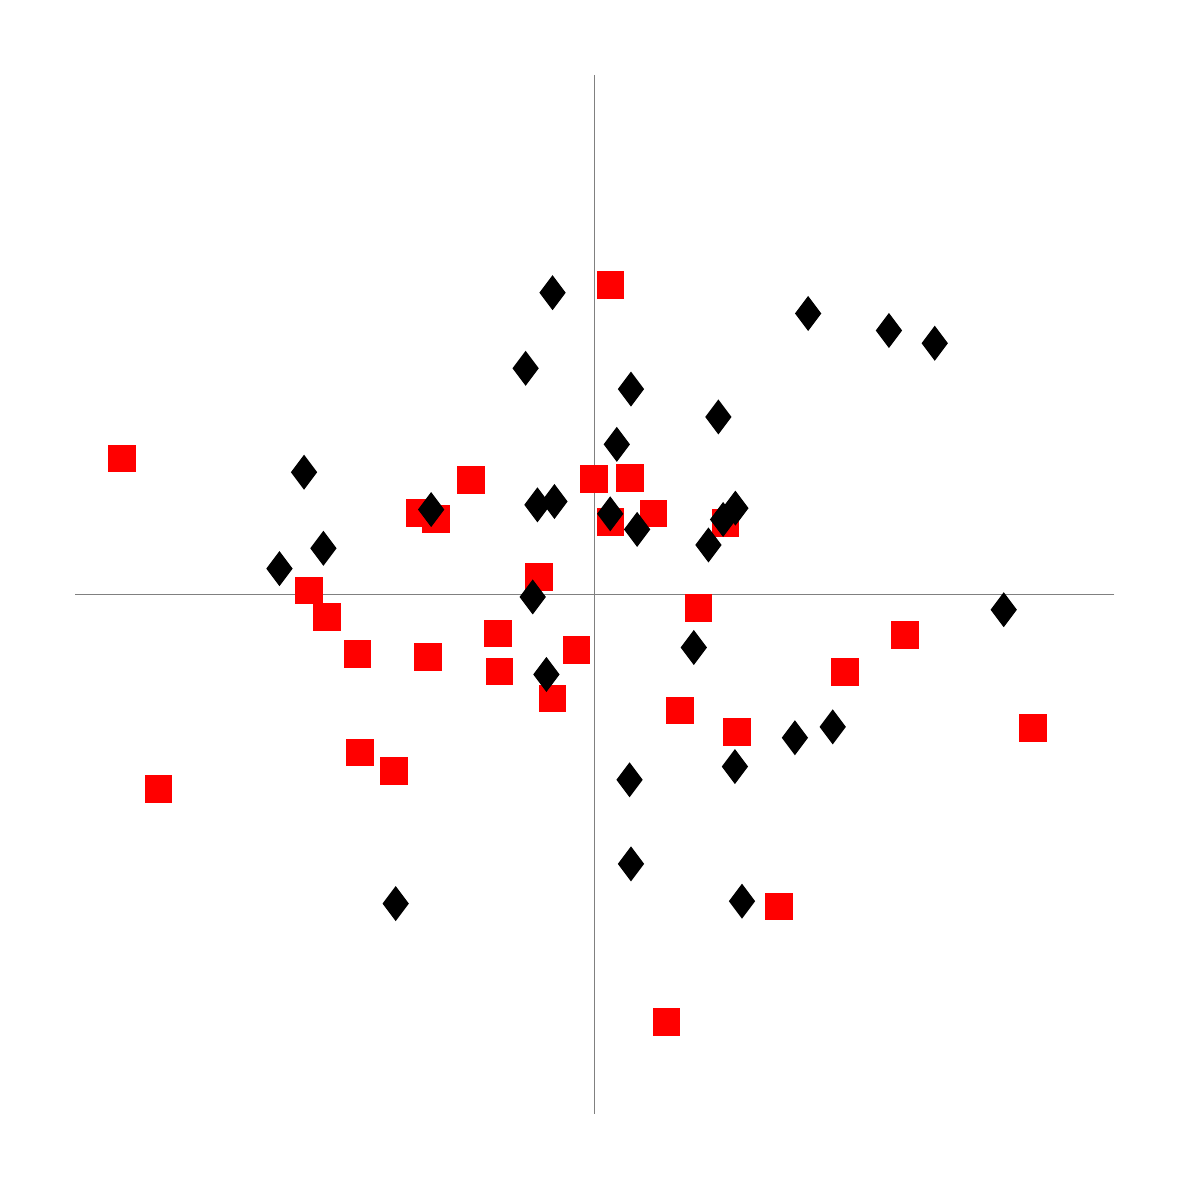
\begin{tikzpicture}[scale=6] \path (-1.2,-1.2) (1.2,1.2);\draw[very thin,color=gray] (0,1.1)--(0,-1.1); \draw[very thin,color=gray] (1.1,0)--(-1.1,0); \path plot[mark=square*,mark options={color=red},mark size=0.8pt] coordinates { (0.530,-0.164) (0.657,-0.086) (-0.352,-0.132) (-0.001,0.244) (-0.201,-0.163) (-0.369,0.173) (0.277,0.152) (-0.923,-0.411) (-0.205,-0.082) (0.034,0.153) (-0.567,-0.047) (-0.118,0.037) (0.125,0.172) (0.390,-0.660) (-0.262,0.243) (0.220,-0.029) (-0.424,-0.374) (-0.496,-0.334) (0.181,-0.245) (-0.335,0.160) (-0.605,0.009) (-1.000,0.288) (0.075,0.247) (-0.502,-0.126) (0.928,-0.283) (-0.038,-0.117) (0.034,0.655) (0.301,-0.291) (-0.089,-0.220) (0.152,-0.905)};  \path plot[mark=diamond*,mark size=1pt] coordinates { (-0.102,-0.169) (-0.089,0.639) (0.074,-0.392) (-0.421,-0.654) (0.504,-0.280) (0.452,0.595) (0.210,-0.112) (0.720,0.532) (-0.085,0.197) (0.047,0.318) (0.312,-0.649) (0.866,-0.032) (0.241,0.105) (0.262,0.376) (-0.667,0.055) (0.297,-0.364) (0.272,0.159) (-0.346,0.180) (0.033,0.171) (0.623,0.559) (-0.131,-0.005) (0.077,0.435) (0.424,-0.303) (-0.615,0.259) (0.298,0.183) (-0.146,0.479) (0.090,0.138) (-0.121,0.190) (-0.574,0.098) (0.077,-0.570)};  \end{tikzpicture} }} & \raisebox{-.5\height}{\resizebox {1.2cm} {1.2cm} { 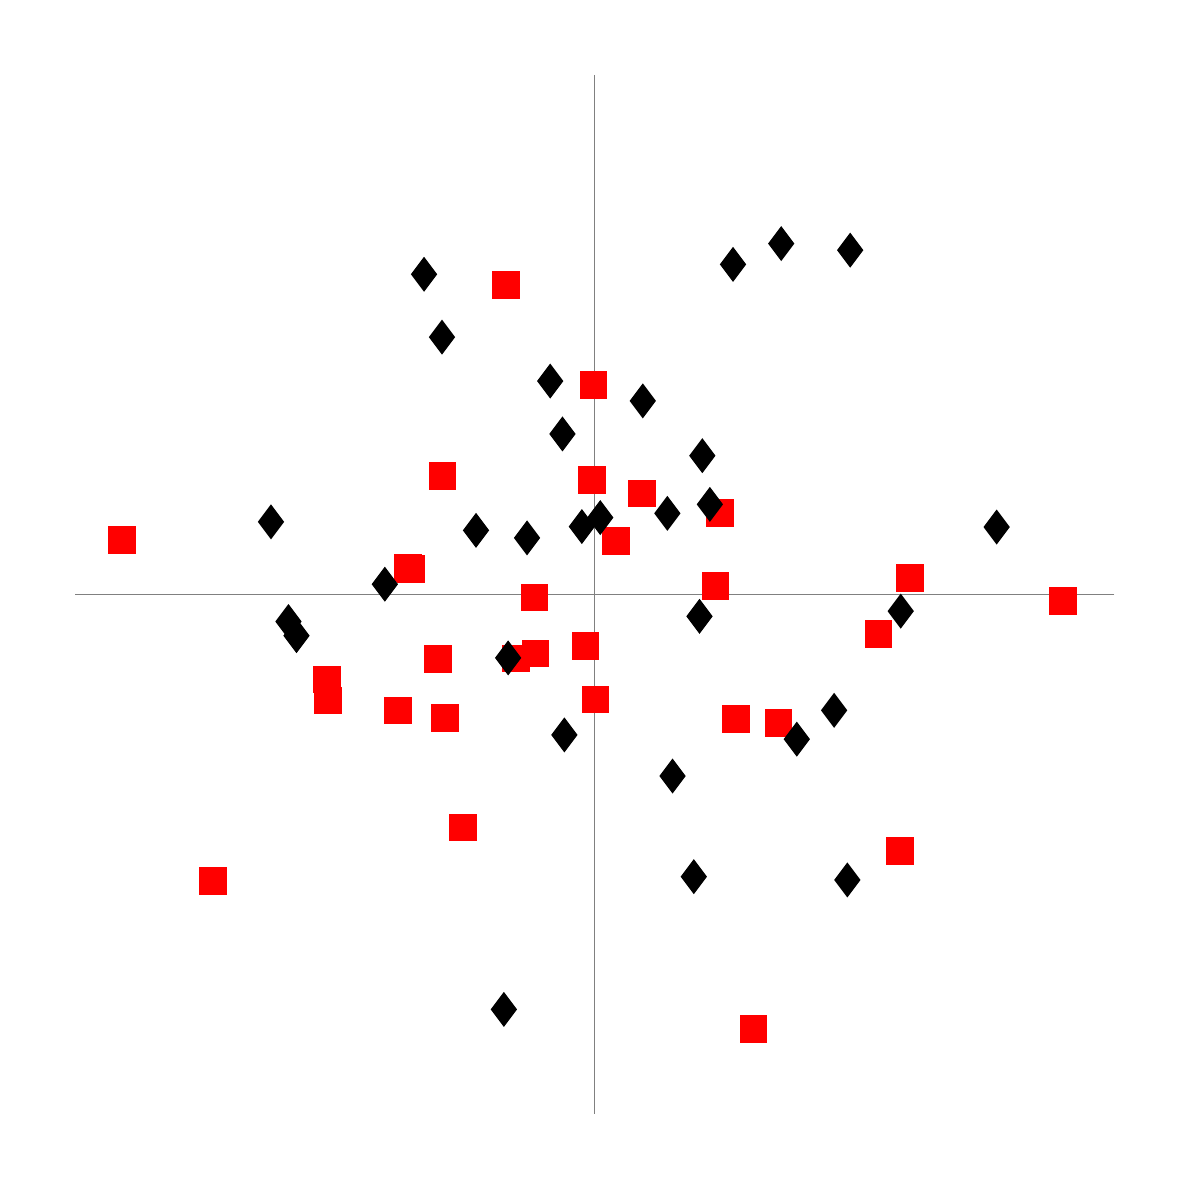
\begin{tikzpicture}[scale=6] \path (-1.2,-1.2) (1.2,1.2);\draw[very thin,color=gray] (0,1.1)--(0,-1.1); \draw[very thin,color=gray] (1.1,0)--(-1.1,0); \path plot[mark=square*,mark options={color=red},mark size=0.8pt] coordinates { (0.601,-0.084) (0.668,0.035) (-0.331,-0.136) (-0.006,0.243) (-0.167,-0.135) (-0.389,0.054) (0.266,0.173) (-0.807,-0.606) (-0.125,-0.125) (0.045,0.114) (-0.564,-0.224) (-0.127,-0.006) (0.100,0.214) (0.646,-0.542) (-0.322,0.251) (0.256,0.018) (-0.279,-0.493) (-0.317,-0.261) (0.299,-0.263) (-0.395,0.056) (-0.566,-0.180) (-1.000,0.115) (-0.002,0.443) (-0.416,-0.245) (0.991,-0.013) (-0.019,-0.109) (-0.188,0.655) (0.389,-0.272) (0.002,-0.222) (0.336,-0.919)};  \path plot[mark=diamond*,mark size=1pt] coordinates { (-0.064,-0.297) (-0.361,0.678) (0.165,-0.384) (-0.192,-0.878) (0.648,-0.035) (0.293,0.699) (0.222,-0.046) (0.541,0.729) (-0.143,0.120) (-0.068,0.340) (0.535,-0.604) (0.851,0.143) (0.154,0.172) (0.102,0.410) (-0.631,-0.087) (0.428,-0.306) (0.244,0.191) (-0.444,0.022) (-0.027,0.144) (0.395,0.743) (-0.183,-0.134) (-0.094,0.452) (0.507,-0.245) (-0.685,0.154) (0.228,0.294) (-0.323,0.545) (0.012,0.163) (-0.251,0.136) (-0.648,-0.057) (0.210,-0.597)};  \end{tikzpicture} }}\\
\midrule
\multirow{4}{*}{III}
 & $\#$PCs & 7 & 1 & 2 & 2 & 20 & 1 & 14\\
 & MNV & \uuline{<1e-08} & * & \uuline{<1e-08} & \uuline{<1e-08} & \uuline{<1e-08} & * & \uuline{<1e-08}\\
 & $t$-test & \uuline{<1e-08} & \uuline{<1e-08} & \uuline{<1e-08} & \uuline{<1e-08} & \uuline{<1e-08} & \uuline{<1e-08} & \uuline{<1e-08}\\
 & PCS & \raisebox{-.5\height}{\resizebox {1.2cm} {1.2cm} { 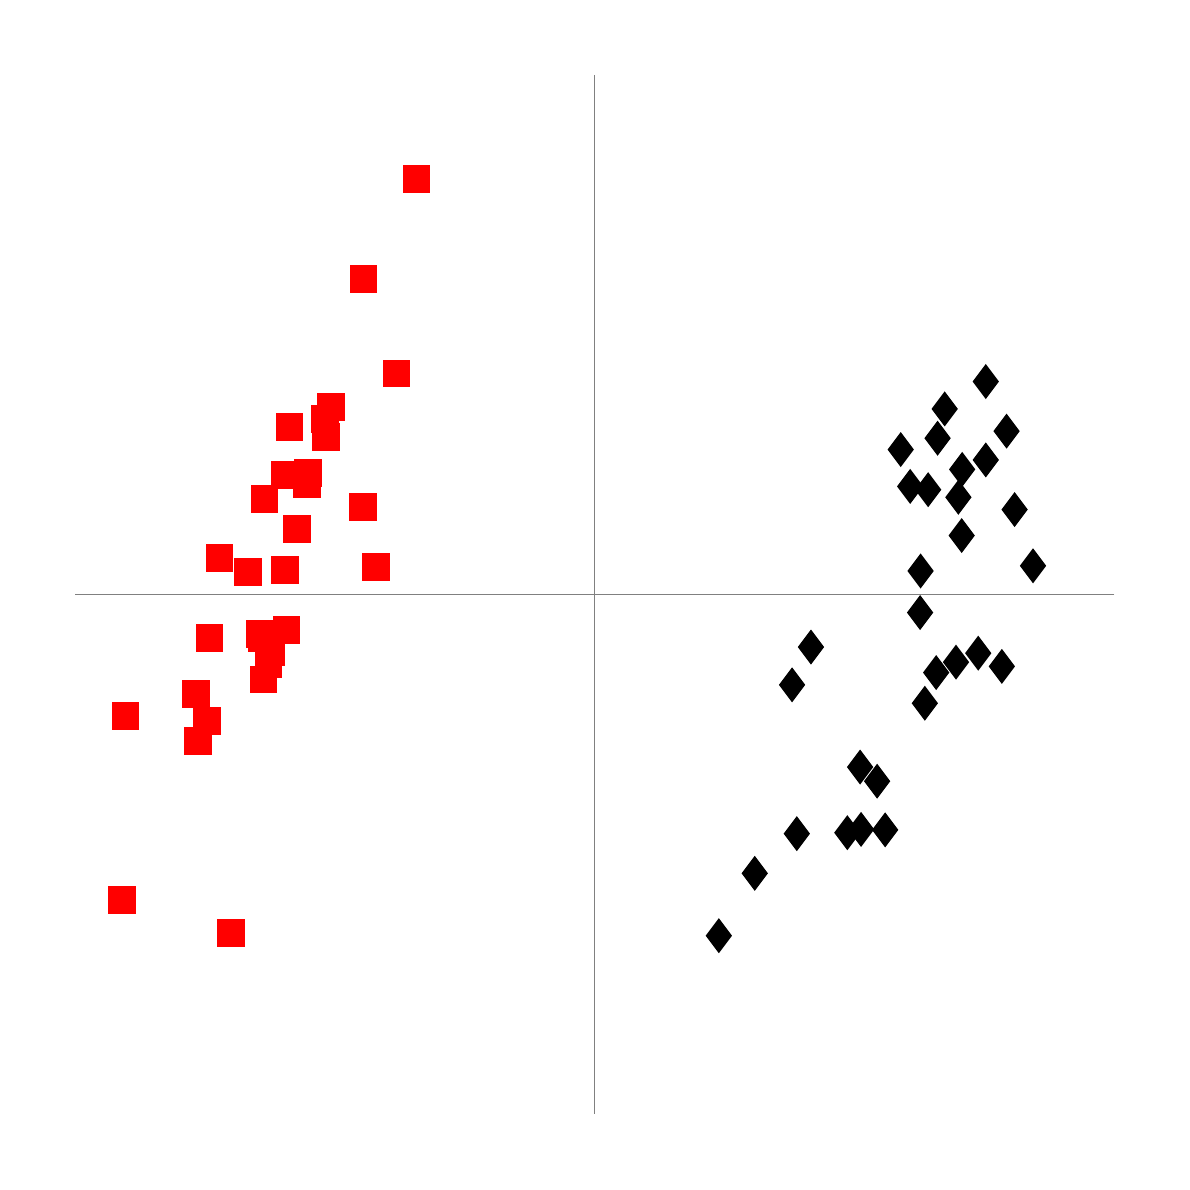
\begin{tikzpicture}[scale=6] \path (-1.2,-1.2) (1.2,1.2);\draw[very thin,color=gray] (0,1.1)--(0,-1.1); \draw[very thin,color=gray] (1.1,0)--(-1.1,0); \path plot[mark=square*,mark options={color=red},mark size=0.8pt] coordinates { (-0.419,0.468) (-0.489,0.668) (-0.690,-0.147) (-0.630,0.139) (-0.704,-0.092) (-0.701,-0.180) (-0.568,0.334) (-1.000,-0.646) (-0.708,-0.084) (-0.462,0.058) (-0.821,-0.268) (-0.655,0.052) (-0.656,0.253) (-0.646,0.355) (-0.652,-0.075) (-0.570,0.371) (-0.815,-0.092) (-0.993,-0.257) (-0.606,0.258) (-0.685,-0.121) (-0.839,-0.310) (-0.770,-0.716) (-0.490,0.186) (-0.843,-0.211) (-0.377,0.880) (-0.733,0.048) (-0.609,0.234) (-0.558,0.397) (-0.794,0.078) (-0.699,0.202)};  \path plot[mark=diamond*,mark size=1pt] coordinates { (0.615,-0.498) (0.812,-0.124) (0.690,0.050) (0.778,0.265) (0.339,-0.590) (0.562,-0.365) (0.706,0.222) (0.535,-0.504) (0.668,0.229) (0.458,-0.111) (0.765,-0.143) (0.699,-0.230) (0.741,0.393) (0.872,0.346) (0.648,0.307) (0.828,0.451) (0.598,-0.395) (0.726,0.331) (0.828,0.285) (0.428,-0.506) (0.263,-0.722) (0.862,-0.152) (0.418,-0.191) (0.928,0.061) (0.770,0.206) (0.564,-0.497) (0.889,0.180) (0.777,0.125) (0.723,-0.165) (0.689,-0.038)};  \end{tikzpicture} }} & \raisebox{-.5\height}{\resizebox {1.2cm} {1.2cm} { \begin{tikzpicture}[scale=6] \path (-1.2,-1.2) (1.2,1.2);\draw[very thin,color=gray] (0,1.1)--(0,-1.1); \draw[very thin,color=gray] (1.1,0)--(-1.1,0); \path plot[mark=square*,mark options={color=red},mark size=0.8pt] coordinates { (-0.751,0.071) (-0.751,-0.042) (-0.903,0.066) (-0.873,0.013) (-0.917,-0.049) (-0.883,0.094) (-0.816,-0.033) (-1.000,0.007) (-0.878,-0.040) (-0.775,0.073) (-0.924,-0.039) (-0.876,0.101) (-0.831,-0.042) (-0.862,-0.142) (-0.865,0.084) (-0.797,-0.072) (-0.922,0.048) (-0.982,-0.007) (-0.842,0.021) (-0.855,-0.016) (-0.916,-0.040) (-0.990,-0.025) (-0.828,-0.027) (-0.958,-0.008) (-0.748,0.012) (-0.853,0.054) (-0.772,-0.102) (-0.842,-0.124) (-0.892,-0.029) (-0.870,0.220)};  \path plot[mark=diamond*,mark size=1pt] coordinates { (0.893,0.001) (0.870,-0.008) (0.867,0.027) (0.925,0.069) (0.762,0.139) (0.851,-0.379) (0.926,-0.171) (0.788,0.036) (0.892,-0.301) (0.804,-0.015) (0.867,0.111) (0.828,-0.272) (0.893,-0.374) (0.940,0.014) (0.940,0.247) (0.886,-0.400) (0.837,0.371) (0.927,0.154) (0.949,-0.002) (0.827,0.383) (0.676,-0.053) (0.930,0.270) (0.782,-0.244) (0.933,0.218) (0.907,0.172) (0.781,-0.012) (0.894,0.243) (0.879,-0.024) (0.829,-0.170) (0.889,-0.052)};  \end{tikzpicture} }} & \raisebox{-.5\height}{\resizebox {1.2cm} {1.2cm} { 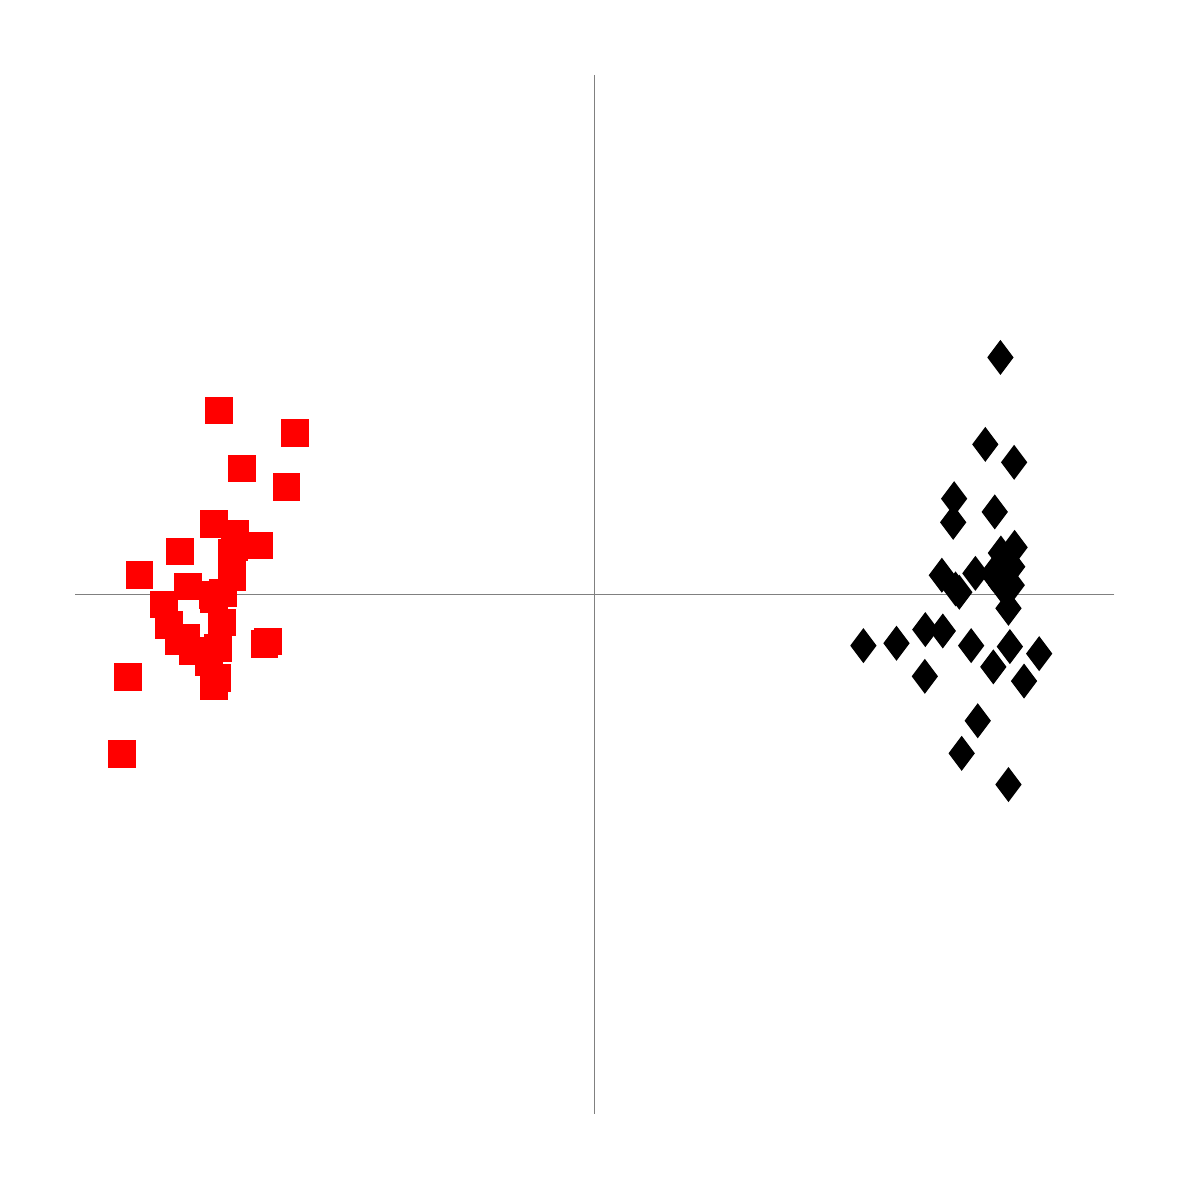
\begin{tikzpicture}[scale=6] \path (-1.2,-1.2) (1.2,1.2);\draw[very thin,color=gray] (0,1.1)--(0,-1.1); \draw[very thin,color=gray] (1.1,0)--(-1.1,0); \path plot[mark=square*,mark options={color=red},mark size=0.8pt] coordinates { (-0.711,0.104) (-0.652,0.228) (-0.850,-0.120) (-0.788,-0.059) (-0.860,0.017) (-0.806,-0.193) (-0.767,0.088) (-0.987,-0.175) (-0.805,-0.010) (-0.699,-0.104) (-0.864,-0.092) (-0.797,-0.113) (-0.767,0.037) (-0.795,0.390) (-0.798,-0.176) (-0.761,0.128) (-0.912,-0.021) (-0.963,0.042) (-0.762,0.101) (-0.816,-0.143) (-0.881,-0.098) (-1.000,-0.338) (-0.787,0.003) (-0.901,-0.064) (-0.634,0.342) (-0.807,-0.001) (-0.691,-0.099) (-0.747,0.267) (-0.877,0.091) (-0.805,0.150)};  \path plot[mark=diamond*,mark size=1pt] coordinates { (0.811,-0.267) (0.797,-0.108) (0.806,0.045) (0.884,0.059) (0.639,-0.103) (0.772,0.005) (0.847,0.175) (0.737,-0.077) (0.827,0.318) (0.761,0.203) (0.844,-0.153) (0.764,0.012) (0.888,0.280) (0.889,0.100) (0.876,-0.029) (0.859,0.502) (0.777,-0.336) (0.883,0.020) (0.941,-0.125) (0.699,-0.173) (0.569,-0.108) (0.876,-0.402) (0.735,0.041) (0.909,-0.183) (0.843,0.044) (0.700,-0.074) (0.860,0.088) (0.861,0.020) (0.759,0.153) (0.879,-0.110)};  \end{tikzpicture} }} & \raisebox{-.5\height}{\resizebox {1.2cm} {1.2cm} { 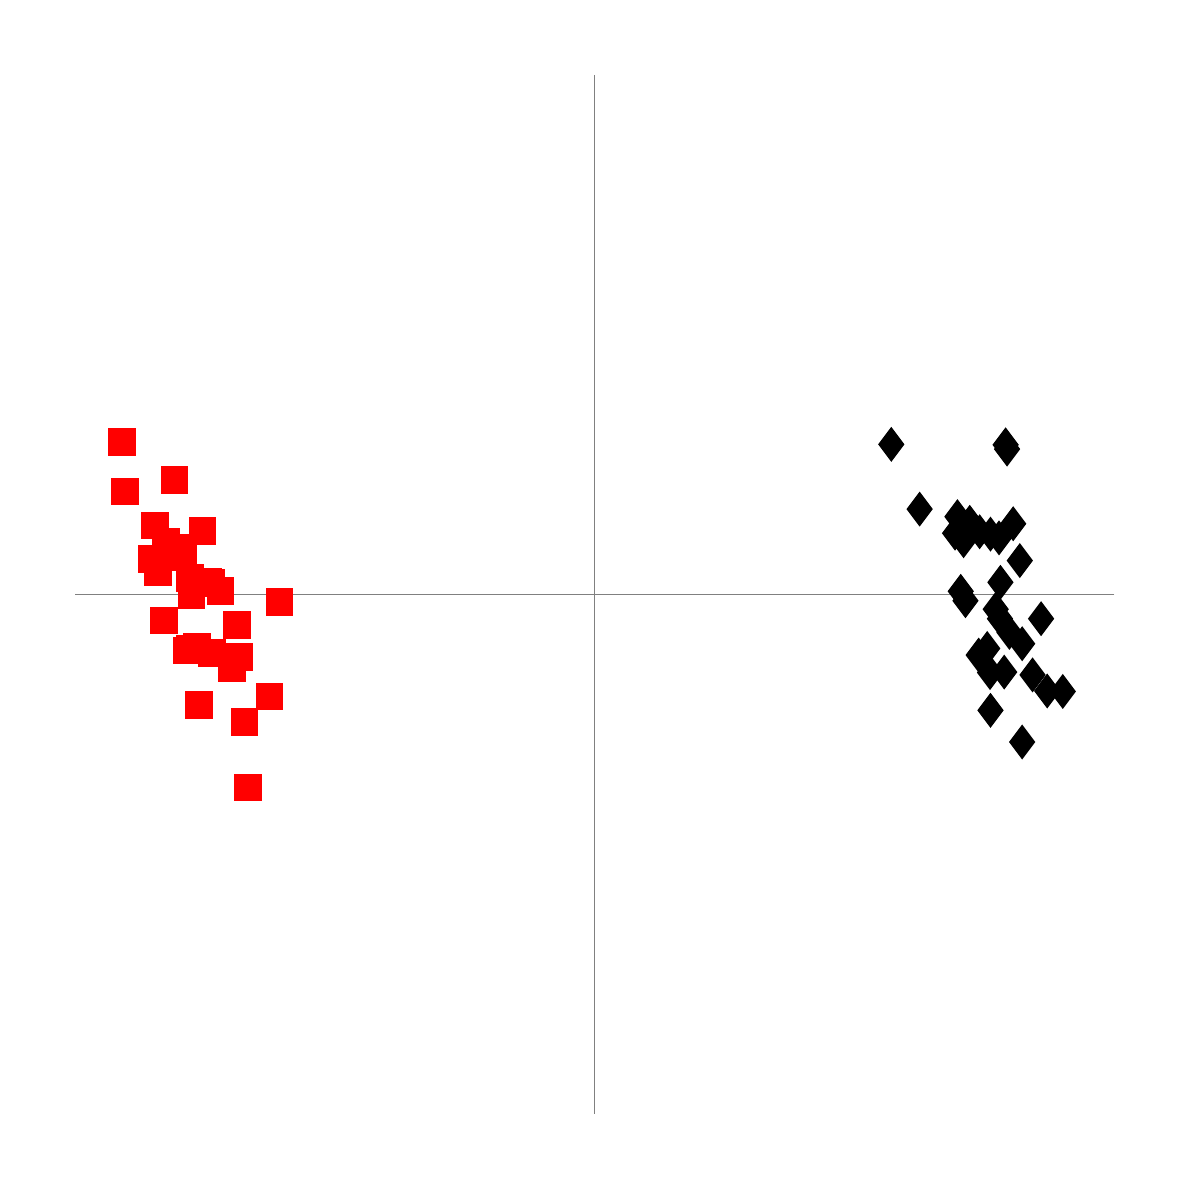
\begin{tikzpicture}[scale=6] \path (-1.2,-1.2) (1.2,1.2);\draw[very thin,color=gray] (0,1.1)--(0,-1.1); \draw[very thin,color=gray] (1.1,0)--(-1.1,0); \path plot[mark=square*,mark options={color=red},mark size=0.8pt] coordinates { (-0.741,-0.270) (-0.688,-0.216) (-0.870,0.079) (-0.853,-0.002) (-0.924,0.048) (-0.886,0.084) (-0.768,-0.156) (-0.994,0.218) (-0.830,0.134) (-0.792,0.008) (-0.907,0.112) (-0.819,0.026) (-0.753,-0.132) (-0.837,-0.234) (-0.856,0.035) (-0.841,-0.111) (-0.882,0.099) (-0.937,0.076) (-0.757,-0.065) (-0.874,0.084) (-0.889,0.242) (-1.000,0.323) (-0.863,-0.118) (-0.931,0.146) (-0.733,-0.408) (-0.811,0.025) (-0.667,-0.015) (-0.810,-0.123) (-0.911,-0.055) (-0.857,-0.115)};  \path plot[mark=diamond*,mark size=1pt] coordinates { (0.873,0.308) (0.785,-0.013) (0.858,-0.051) (0.905,-0.104) (0.688,0.181) (0.870,0.317) (0.878,-0.080) (0.838,0.128) (0.831,-0.114) (0.900,0.072) (0.886,0.150) (0.781,0.114) (0.991,-0.205) (0.958,-0.204) (0.927,-0.170) (0.838,-0.245) (0.768,0.165) (0.837,-0.165) (0.945,-0.051) (0.794,0.153) (0.628,0.318) (0.856,0.120) (0.815,0.133) (0.849,-0.031) (0.867,-0.164) (0.763,0.130) (0.905,-0.312) (0.813,-0.128) (0.775,0.007) (0.859,0.026)};  \end{tikzpicture} }} & \raisebox{-.5\height}{\resizebox {1.2cm} {1.2cm} { 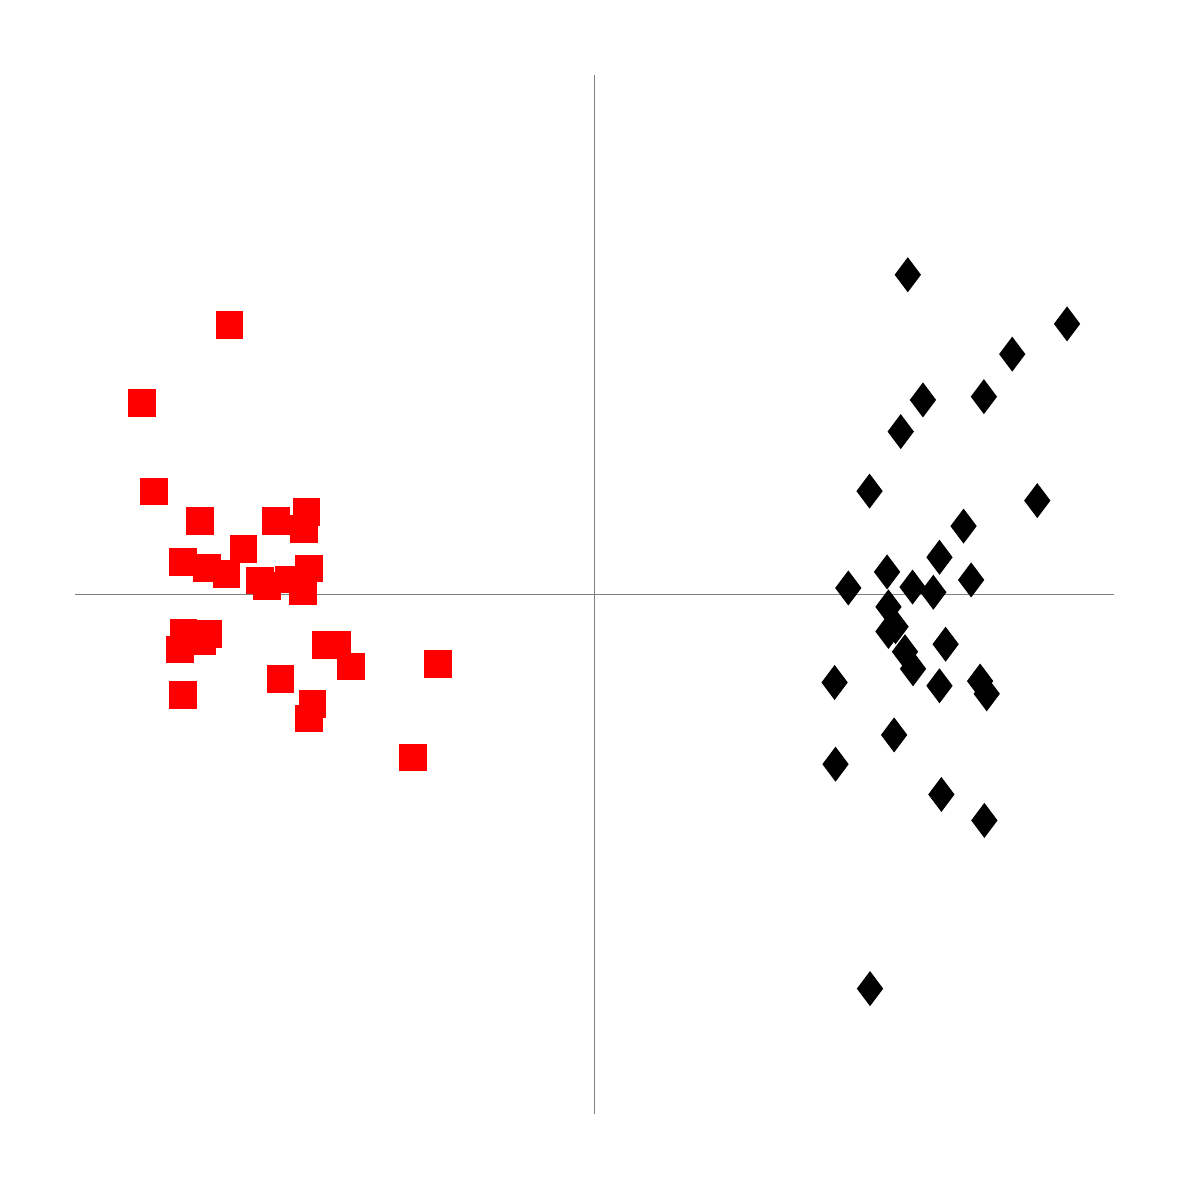
\begin{tikzpicture}[scale=6] \path (-1.2,-1.2) (1.2,1.2);\draw[very thin,color=gray] (0,1.1)--(0,-1.1); \draw[very thin,color=gray] (1.1,0)--(-1.1,0); \path plot[mark=square*,mark options={color=red},mark size=0.8pt] coordinates { (-0.544,-0.107) (-0.870,-0.080) (-0.871,-0.213) (-0.694,0.018) (-0.605,0.055) (-0.597,-0.232) (-0.610,0.175) (-0.617,0.007) (-0.515,-0.152) (-0.332,-0.147) (-0.852,-0.082) (-0.708,0.030) (-0.743,0.097) (-0.773,0.571) (-0.665,-0.178) (-0.871,0.069) (-0.818,-0.084) (-0.830,-0.098) (-0.933,0.218) (-0.674,0.156) (-0.615,0.139) (-0.385,-0.345) (-0.568,-0.107) (-0.648,0.032) (-0.779,0.044) (-0.878,-0.116) (-0.820,0.056) (-0.958,0.405) (-0.835,0.156) (-0.605,-0.262)};  \path plot[mark=diamond*,mark size=1pt] coordinates { (0.730,-0.193) (0.622,-0.026) (0.619,0.048) (0.673,0.016) (0.743,-0.105) (0.884,0.509) (0.582,0.219) (0.510,-0.359) (0.824,0.419) (0.648,0.345) (0.637,-0.068) (0.781,0.145) (0.663,0.677) (0.537,0.014) (0.634,-0.297) (1.000,0.573) (0.583,-0.834) (0.674,-0.157) (0.717,0.005) (0.734,-0.423) (0.937,0.199) (0.825,-0.478) (0.695,0.412) (0.830,-0.210) (0.797,0.031) (0.657,-0.121) (0.816,-0.183) (0.622,-0.078) (0.730,0.079) (0.508,-0.186)};  \end{tikzpicture} }} & \raisebox{-.5\height}{\resizebox {1.2cm} {1.2cm} { \begin{tikzpicture}[scale=6] \path (-1.2,-1.2) (1.2,1.2);\draw[very thin,color=gray] (0,1.1)--(0,-1.1); \draw[very thin,color=gray] (1.1,0)--(-1.1,0); \path plot[mark=square*,mark options={color=red},mark size=0.8pt] coordinates { (-0.874,0.094) (-0.841,0.132) (-0.929,-0.046) (-0.901,-0.022) (-0.933,-0.009) (-0.904,-0.087) (-0.897,0.052) (-0.976,-0.133) (-0.904,-0.028) (-0.868,-0.039) (-0.928,-0.077) (-0.903,-0.034) (-0.889,0.015) (-0.902,0.167) (-0.904,-0.070) (-0.893,0.070) (-0.951,-0.017) (-0.964,-0.014) (-0.889,0.064) (-0.912,-0.080) (-0.935,-0.087) (-1.000,-0.202) (-0.911,0.014) (-0.943,-0.053) (-0.840,0.225) (-0.903,-0.000) (-0.854,-0.053) (-0.885,0.122) (-0.935,0.034) (-0.905,0.112)};  \path plot[mark=diamond*,mark size=1pt] coordinates { (0.912,-0.148) (0.894,-0.044) (0.906,0.032) (0.935,0.061) (0.850,-0.056) (0.897,-0.078) (0.922,0.063) (0.884,-0.056) (0.918,0.106) (0.901,0.070) (0.918,-0.047) (0.887,-0.042) (0.942,0.093) (0.934,0.072) (0.943,0.038) (0.923,0.186) (0.898,-0.104) (0.939,0.052) (0.959,-0.024) (0.875,-0.051) (0.824,-0.091) (0.927,-0.127) (0.890,-0.032) (0.938,-0.029) (0.919,0.061) (0.867,-0.062) (0.920,0.097) (0.928,0.016) (0.884,0.037) (0.940,-0.045)};  \end{tikzpicture} }} & \raisebox{-.5\height}{\resizebox {1.2cm} {1.2cm} { 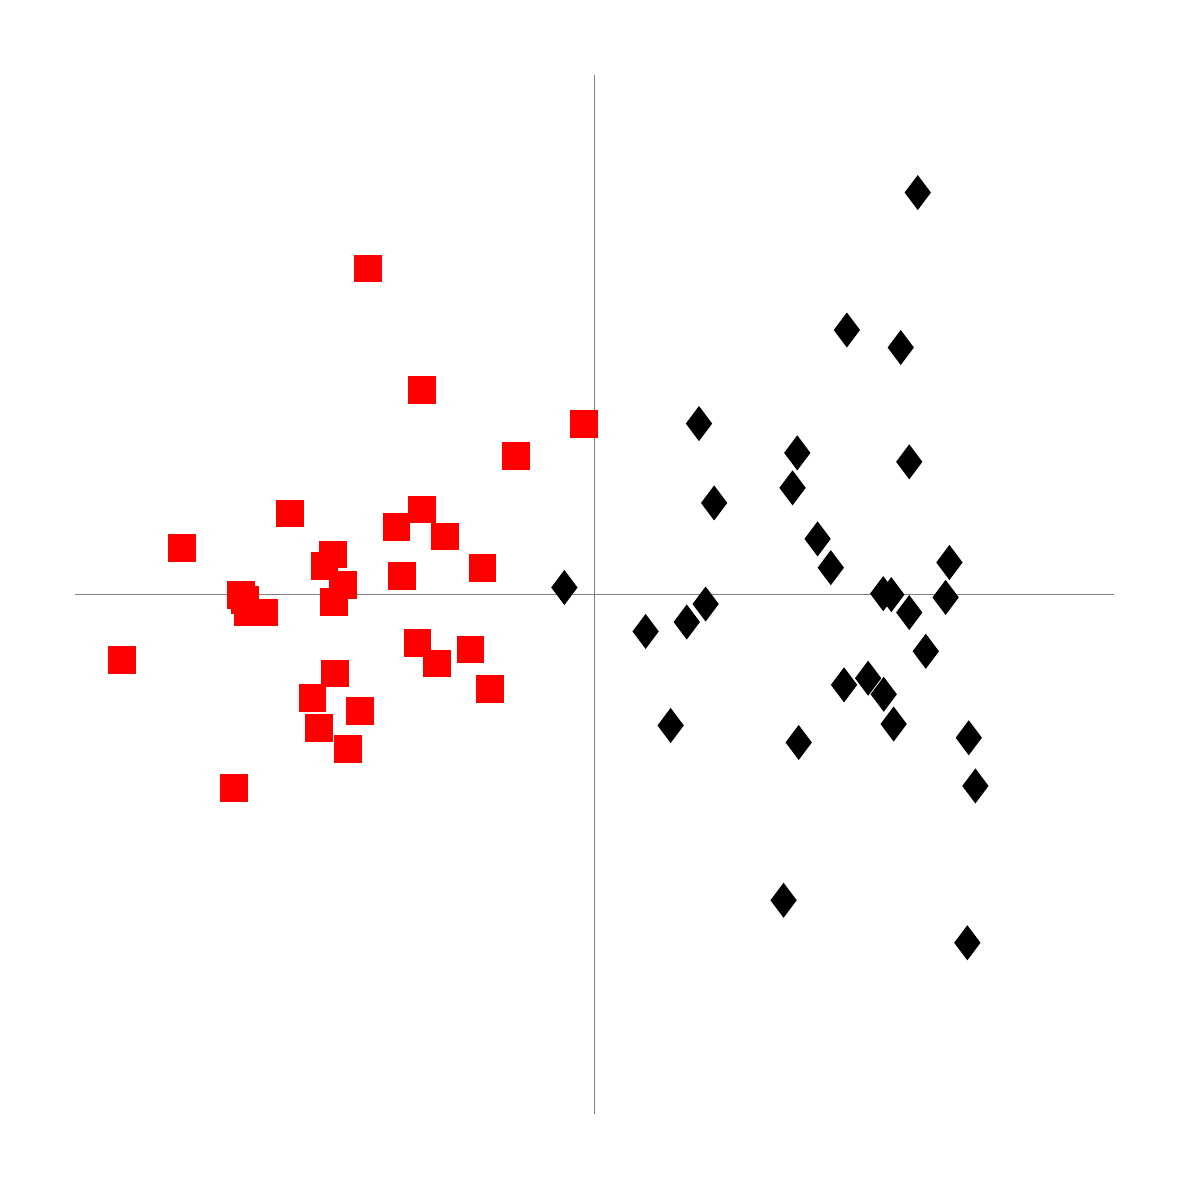
\begin{tikzpicture}[scale=6] \path (-1.2,-1.2) (1.2,1.2);\draw[very thin,color=gray] (0,1.1)--(0,-1.1); \draw[very thin,color=gray] (1.1,0)--(-1.1,0); \path plot[mark=square*,mark options={color=red},mark size=0.8pt] coordinates { (-0.237,0.056) (-0.167,0.294) (-0.597,-0.219) (-0.375,-0.103) (-0.572,0.060) (-0.583,-0.282) (-0.316,0.123) (-1.000,-0.138) (-0.533,0.021) (-0.222,-0.200) (-0.734,-0.038) (-0.497,-0.246) (-0.408,0.039) (-0.480,0.690) (-0.522,-0.327) (-0.366,0.180) (-0.699,-0.038) (-0.874,0.098) (-0.419,0.143) (-0.550,-0.167) (-0.740,-0.011) (-0.763,-0.410) (-0.263,-0.116) (-0.748,-0.001) (-0.022,0.361) (-0.551,-0.015) (-0.333,-0.146) (-0.365,0.433) (-0.645,0.172) (-0.554,0.085)};  \path plot[mark=diamond*,mark size=1pt] coordinates { (0.432,-0.313) (0.612,-0.211) (0.500,0.057) (0.743,-0.006) (0.108,-0.078) (0.419,0.226) (0.666,0.281) (0.195,-0.058) (0.534,0.560) (0.221,0.362) (0.633,-0.274) (0.472,0.118) (0.648,0.523) (0.751,0.068) (0.579,-0.177) (0.684,0.851) (0.400,-0.647) (0.701,-0.120) (0.792,-0.303) (0.161,-0.277) (-0.064,0.015) (0.789,-0.737) (0.253,0.194) (0.806,-0.405) (0.611,0.002) (0.235,-0.020) (0.666,-0.038) (0.628,-0.000) (0.429,0.300) (0.528,-0.191)};  \end{tikzpicture} }}\\
\bottomrule
\end{tabular}
} % resize box
\end{table}
\end{document}
